\documentclass[uplatex,dvipdfmx]{jsreport}
\title{今日の圏論}
\author{司馬博文}
\date{\today}
\pagestyle{headings} \setcounter{secnumdepth}{4}
%%%%%%%%%%%%%%%% 数理文書の組版 %%%%%%%%%%%%%%%

\usepackage{mathtools} %内部でamsmathを呼び出すことに注意.
%\mathtoolsset{showonlyrefs=true} %labelを附した数式にのみ附番される設定.
\usepackage{amsfonts} %mathfrak, mathcal, mathbbなど.
\usepackage{amsthm} %定理環境.
\usepackage{amssymb} %AMSFontsを使うためのパッケージ.
\usepackage{ascmac} %screen, itembox, shadebox環境.全てLATEX2εの標準機能の範囲で作られたもの.
\usepackage{comment} %comment環境を用いて,複数行をcomment outできるようにするpackage
\usepackage{wrapfig} %図の周りに文字をwrapさせることができる.詳細な制御ができる.
\usepackage[usenames, dvipsnames]{xcolor} %xcolorはcolorの拡張.optionの意味はdvipsnamesはLoad a set of predefined colors. forestgreenなどの色が追加されている.usenamesはobsoleteとだけ書いてあった.
\setcounter{tocdepth}{2} %目次に表示される深さ.2はsubsectionまで
\usepackage{multicol} %\begin{multicols}{2}環境で途中からmulticolumnに出来る.
\usepackage{mathabx}\newcommand{\wc}{\widecheck} %\widecheckなどのフォントパッケージ

%%%%%%%%%%%%%%% フォント %%%%%%%%%%%%%%%

\usepackage{textcomp, mathcomp} %Text Companionとは,T1 encodingに入らなかった文字群.これを使うためのパッケージ.\textsectionでブルバキに!
\usepackage[T1]{fontenc} %8bitエンコーディングにする.comp系拡張数学文字の動作が安定する.

%%%%%%%%%%%%%%% 一般文書の組版 %%%%%%%%%%%%%%%

\definecolor{花緑青}{cmyk}{1,0.07,0.10,0.10}\definecolor{サーモンピンク}{cmyk}{0,0.65,0.65,0.05}\definecolor{暗中模索}{rgb}{0.2,0.2,0.2}
\usepackage{url}\usepackage[dvipdfmx,colorlinks,linkcolor=花緑青,urlcolor=花緑青,citecolor=花緑青]{hyperref} %生成されるPDFファイルにおいて、\tableofcontentsによって書き出された目次をクリックすると該当する見出しへジャンプしたり、さらには、\label{ラベル名}を番号で参照する\ref{ラベル名}やthebibliography環境において\bibitem{ラベル名}を文献番号で参照する\cite{ラベル名}においても番号をクリックすると該当箇所にジャンプする.囲み枠はダサいので,colorlinksで囲み廃止し,リンク自体に色を付けることにした.
\usepackage{pxjahyper} %pxrubrica同様,八登崇之さん.hyperrefは日本語pLaTeXに最適化されていないから,hyperrefとセットで,(u)pLaTeX+hyperref+dvipdfmxの組み合わせで日本語を含む「しおり」をもつPDF文書を作成する場合に必要となる機能を提供する
\usepackage{ulem} %取り消し線を引くためのパッケージ
\usepackage{pxrubrica} %日本語にルビをふる.八登崇之(やとうたかゆき)氏による.

%%%%%%%%%%%%%%% 科学文書の組版 %%%%%%%%%%%%%%%

\usepackage[version=4]{mhchem} %化学式をTikZで簡単に書くためのパッケージ.
\usepackage{chemfig} %化学構造式をTikZで描くためのパッケージ.
\usepackage{siunitx} %IS単位を書くためのパッケージ

%%%%%%%%%%%%%%% 作図 %%%%%%%%%%%%%%%

\usepackage{tikz}\usetikzlibrary{positioning,automata}\usepackage{tikz-cd}\usepackage[all]{xy}
\def\objectstyle{\displaystyle} %デフォルトではxymatrix中の数式が文中数式モードになるので,それを直す.\labelstyleも同様にxy packageの中で定義されており,文中数式モードになっている.

\usepackage{graphicx} %rotatebox, scalebox, reflectbox, resizeboxなどのコマンドや,図表の読み込み\includegraphicsを司る.graphics というパッケージもありますが,graphicx はこれを高機能にしたものと考えて結構です(ただし graphicx は内部で graphics を読み込みます)
\usepackage[top=15truemm,bottom=15truemm,left=10truemm,right=10truemm]{geometry} %足助さんからもらったオプション

%%%%%%%%%%%%%%% 参照 %%%%%%%%%%%%%%%
%参考文献リストを出力したい箇所に\bibliography{../mathematics.bib}を追記すると良い.

%\bibliographystyle{jplain}
%\bibliographystyle{jname}
\bibliographystyle{apalike}

%%%%%%%%%%%%%%% 計算機文書の組版 %%%%%%%%%%%%%%%

\usepackage[breakable]{tcolorbox} %加藤晃史さんがフル活用していたtcolorboxを,途中改ページ可能で.
\tcbuselibrary{theorems} %https://qiita.com/t_kemmochi/items/483b8fcdb5db8d1f5d5e
\usepackage{enumerate} %enumerate環境を凝らせる.

\usepackage{listings} %ソースコードを表示できる環境.多分もっといい方法ある.
\usepackage{jvlisting} %日本語のコメントアウトをする場合jlistingが必要
\lstset{ %ここからソースコードの表示に関する設定.lstlisting環境では,[caption=hoge,label=fuga]などのoptionを付けられる.
%[escapechar=!]とすると,LaTeXコマンドを使える.
  basicstyle={\ttfamily},
  identifierstyle={\small},
  commentstyle={\smallitshape},
  keywordstyle={\small\bfseries},
  ndkeywordstyle={\small},
  stringstyle={\small\ttfamily},
  frame={tb},
  breaklines=true,
  columns=[l]{fullflexible},
  numbers=left,
  xrightmargin=0zw,
  xleftmargin=3zw,
  numberstyle={\scriptsize},
  stepnumber=1,
  numbersep=1zw,
  lineskip=-0.5ex
}
%\makeatletter %caption番号を「[chapter番号].[section番号].[subsection番号]-[そのsubsection内においてn番目]」に変更
%    \AtBeginDocument{
%    \renewcommand*{\thelstlisting}{\arabic{chapter}.\arabic{section}.\arabic{lstlisting}}
%    \@addtoreset{lstlisting}{section}
%    }
%\makeatother
\renewcommand{\lstlistingname}{算譜} %caption名を"program"に変更

\newtcolorbox{tbox}[3][]{%
colframe=#2,colback=#2!10,coltitle=#2!20!black,title={#3},#1}

% 証明内の文字が小さくなる環境.
\newenvironment{Proof}[1][\bf\underline{[証明]}]{\proof[#1]\color{darkgray}}{\endproof}

%%%%%%%%%%%%%%% 数学記号のマクロ %%%%%%%%%%%%%%%

%%% 括弧類
\newcommand{\abs}[1]{\lvert#1\rvert}\newcommand{\Abs}[1]{\left|#1\right|}\newcommand{\norm}[1]{\|#1\|}\newcommand{\Norm}[1]{\left\|#1\right\|}\newcommand{\Brace}[1]{\left\{#1\right\}}\newcommand{\BRace}[1]{\biggl\{#1\biggr\}}\newcommand{\paren}[1]{\left(#1\right)}\newcommand{\Paren}[1]{\biggr(#1\biggl)}\newcommand{\bracket}[1]{\langle#1\rangle}\newcommand{\brac}[1]{\langle#1\rangle}\newcommand{\Bracket}[1]{\left\langle#1\right\rangle}\newcommand{\Brac}[1]{\left\langle#1\right\rangle}\newcommand{\bra}[1]{\left\langle#1\right|}\newcommand{\ket}[1]{\left|#1\right\rangle}\newcommand{\Square}[1]{\left[#1\right]}\newcommand{\SQuare}[1]{\biggl[#1\biggr]}
\renewcommand{\o}[1]{\overline{#1}}\renewcommand{\u}[1]{\underline{#1}}\newcommand{\wt}[1]{\widetilde{#1}}\newcommand{\wh}[1]{\widehat{#1}}
\newcommand{\pp}[2]{\frac{\partial #1}{\partial #2}}\newcommand{\ppp}[3]{\frac{\partial #1}{\partial #2\partial #3}}\newcommand{\dd}[2]{\frac{d #1}{d #2}}
\newcommand{\floor}[1]{\lfloor#1\rfloor}\newcommand{\Floor}[1]{\left\lfloor#1\right\rfloor}\newcommand{\ceil}[1]{\lceil#1\rceil}
\newcommand{\ocinterval}[1]{(#1]}\newcommand{\cointerval}[1]{[#1)}\newcommand{\COinterval}[1]{\left[#1\right)}


%%% 予約語
\renewcommand{\iff}{\;\mathrm{iff}\;}
\newcommand{\False}{\mathrm{False}}\newcommand{\True}{\mathrm{True}}
\newcommand{\otherwise}{\mathrm{otherwise}}
\newcommand{\st}{\;\mathrm{s.t.}\;}

%%% 略記
\newcommand{\M}{\mathcal{M}}\newcommand{\cF}{\mathcal{F}}\newcommand{\cD}{\mathcal{D}}\newcommand{\fX}{\mathfrak{X}}\newcommand{\fY}{\mathfrak{Y}}\newcommand{\fZ}{\mathfrak{Z}}\renewcommand{\H}{\mathcal{H}}\newcommand{\fH}{\mathfrak{H}}\newcommand{\bH}{\mathbb{H}}\newcommand{\id}{\mathrm{id}}\newcommand{\A}{\mathcal{A}}\newcommand{\U}{\mathfrak{U}}
\newcommand{\lmd}{\lambda}
\newcommand{\Lmd}{\Lambda}

%%% 矢印類
\newcommand{\iso}{\xrightarrow{\,\smash{\raisebox{-0.45ex}{\ensuremath{\scriptstyle\sim}}}\,}}
\newcommand{\Lrarrow}{\;\;\Leftrightarrow\;\;}

%%% 注記
\newcommand{\rednote}[1]{\textcolor{red}{#1}}

% ノルム位相についての閉包 https://newbedev.com/how-to-make-double-overline-with-less-vertical-displacement
\makeatletter
\newcommand{\dbloverline}[1]{\overline{\dbl@overline{#1}}}
\newcommand{\dbl@overline}[1]{\mathpalette\dbl@@overline{#1}}
\newcommand{\dbl@@overline}[2]{%
  \begingroup
  \sbox\z@{$\m@th#1\overline{#2}$}%
  \ht\z@=\dimexpr\ht\z@-2\dbl@adjust{#1}\relax
  \box\z@
  \ifx#1\scriptstyle\kern-\scriptspace\else
  \ifx#1\scriptscriptstyle\kern-\scriptspace\fi\fi
  \endgroup
}
\newcommand{\dbl@adjust}[1]{%
  \fontdimen8
  \ifx#1\displaystyle\textfont\else
  \ifx#1\textstyle\textfont\else
  \ifx#1\scriptstyle\scriptfont\else
  \scriptscriptfont\fi\fi\fi 3
}
\makeatother
\newcommand{\oo}[1]{\dbloverline{#1}}

% hslashの他の文字Ver.
\newcommand{\hslashslash}{%
    \scalebox{1.2}{--
    }%
}
\newcommand{\dslash}{%
  {%
    \vphantom{d}%
    \ooalign{\kern.05em\smash{\hslashslash}\hidewidth\cr$d$\cr}%
    \kern.05em
  }%
}
\newcommand{\dint}{%
  {%
    \vphantom{d}%
    \ooalign{\kern.05em\smash{\hslashslash}\hidewidth\cr$\int$\cr}%
    \kern.05em
  }%
}
\newcommand{\dL}{%
  {%
    \vphantom{d}%
    \ooalign{\kern.05em\smash{\hslashslash}\hidewidth\cr$L$\cr}%
    \kern.05em
  }%
}

%%% 演算子
\DeclareMathOperator{\grad}{\mathrm{grad}}\DeclareMathOperator{\rot}{\mathrm{rot}}\DeclareMathOperator{\divergence}{\mathrm{div}}\DeclareMathOperator{\tr}{\mathrm{tr}}\newcommand{\pr}{\mathrm{pr}}
\newcommand{\Map}{\mathrm{Map}}\newcommand{\dom}{\mathrm{Dom}\;}\newcommand{\cod}{\mathrm{Cod}\;}\newcommand{\supp}{\mathrm{supp}\;}


%%% 線型代数学
\newcommand{\vctr}[2]{\begin{pmatrix}#1\\#2\end{pmatrix}}\newcommand{\vctrr}[3]{\begin{pmatrix}#1\\#2\\#3\end{pmatrix}}\newcommand{\mtrx}[4]{\begin{pmatrix}#1&#2\\#3&#4\end{pmatrix}}\newcommand{\smtrx}[4]{\paren{\begin{smallmatrix}#1&#2\\#3&#4\end{smallmatrix}}}\newcommand{\Ker}{\mathrm{Ker}\;}\newcommand{\Coker}{\mathrm{Coker}\;}\newcommand{\Coim}{\mathrm{Coim}\;}\DeclareMathOperator{\rank}{\mathrm{rank}}\newcommand{\lcm}{\mathrm{lcm}}\newcommand{\sgn}{\mathrm{sgn}\,}\newcommand{\GL}{\mathrm{GL}}\newcommand{\SL}{\mathrm{SL}}\newcommand{\alt}{\mathrm{alt}}
%%% 複素解析学
\renewcommand{\Re}{\mathrm{Re}\;}\renewcommand{\Im}{\mathrm{Im}\;}\newcommand{\Gal}{\mathrm{Gal}}\newcommand{\PGL}{\mathrm{PGL}}\newcommand{\PSL}{\mathrm{PSL}}\newcommand{\Log}{\mathrm{Log}\,}\newcommand{\Res}{\mathrm{Res}\,}\newcommand{\on}{\mathrm{on}\;}\newcommand{\hatC}{\widehat{\C}}\newcommand{\hatR}{\hat{\R}}\newcommand{\PV}{\mathrm{P.V.}}\newcommand{\diam}{\mathrm{diam}}\newcommand{\Area}{\mathrm{Area}}\newcommand{\Lap}{\Laplace}\newcommand{\f}{\mathbf{f}}\newcommand{\cR}{\mathcal{R}}\newcommand{\const}{\mathrm{const.}}\newcommand{\Om}{\Omega}\newcommand{\Cinf}{C^\infty}\newcommand{\ep}{\epsilon}\newcommand{\dist}{\mathrm{dist}}\newcommand{\opart}{\o{\partial}}\newcommand{\Length}{\mathrm{Length}}
%%% 集合と位相
\renewcommand{\O}{\mathcal{O}}\renewcommand{\S}{\mathcal{S}}\renewcommand{\U}{\mathcal{U}}\newcommand{\V}{\mathcal{V}}\renewcommand{\P}{\mathcal{P}}\newcommand{\R}{\mathbb{R}}\newcommand{\N}{\mathbb{N}}\newcommand{\C}{\mathbb{C}}\newcommand{\Z}{\mathbb{Z}}\newcommand{\Q}{\mathbb{Q}}\newcommand{\TV}{\mathrm{TV}}\newcommand{\ORD}{\mathrm{ORD}}\newcommand{\Tr}{\mathrm{Tr}}\newcommand{\Card}{\mathrm{Card}\;}\newcommand{\Top}{\mathrm{Top}}\newcommand{\Disc}{\mathrm{Disc}}\newcommand{\Codisc}{\mathrm{Codisc}}\newcommand{\CoDisc}{\mathrm{CoDisc}}\newcommand{\Ult}{\mathrm{Ult}}\newcommand{\ord}{\mathrm{ord}}\newcommand{\maj}{\mathrm{maj}}\newcommand{\bS}{\mathbb{S}}\newcommand{\PConn}{\mathrm{PConn}}

%%% 形式言語理論
\newcommand{\REGEX}{\mathrm{REGEX}}\newcommand{\RE}{\mathbf{RE}}
%%% Graph Theory
\newcommand{\SimpGph}{\mathrm{SimpGph}}\newcommand{\Gph}{\mathrm{Gph}}\newcommand{\mult}{\mathrm{mult}}\newcommand{\inv}{\mathrm{inv}}

%%% 多様体
\newcommand{\Der}{\mathrm{Der}}\newcommand{\osub}{\overset{\mathrm{open}}{\subset}}\newcommand{\osup}{\overset{\mathrm{open}}{\supset}}\newcommand{\al}{\alpha}\newcommand{\K}{\mathbb{K}}\newcommand{\Sp}{\mathrm{Sp}}\newcommand{\g}{\mathfrak{g}}\newcommand{\h}{\mathfrak{h}}\newcommand{\Exp}{\mathrm{Exp}\;}\newcommand{\Imm}{\mathrm{Imm}}\newcommand{\Imb}{\mathrm{Imb}}\newcommand{\codim}{\mathrm{codim}\;}\newcommand{\Gr}{\mathrm{Gr}}
%%% 代数
\newcommand{\Ad}{\mathrm{Ad}}\newcommand{\finsupp}{\mathrm{fin\;supp}}\newcommand{\SO}{\mathrm{SO}}\newcommand{\SU}{\mathrm{SU}}\newcommand{\acts}{\curvearrowright}\newcommand{\mono}{\hookrightarrow}\newcommand{\epi}{\twoheadrightarrow}\newcommand{\Stab}{\mathrm{Stab}}\newcommand{\nor}{\mathrm{nor}}\newcommand{\T}{\mathbb{T}}\newcommand{\Aff}{\mathrm{Aff}}\newcommand{\rsub}{\triangleleft}\newcommand{\rsup}{\triangleright}\newcommand{\subgrp}{\overset{\mathrm{subgrp}}{\subset}}\newcommand{\Ext}{\mathrm{Ext}}\newcommand{\sbs}{\subset}\newcommand{\sps}{\supset}\newcommand{\In}{\mathrm{in}\;}\newcommand{\Tor}{\mathrm{Tor}}\newcommand{\p}{\b{p}}\newcommand{\q}{\mathfrak{q}}\newcommand{\m}{\mathfrak{m}}\newcommand{\cS}{\mathcal{S}}\newcommand{\Frac}{\mathrm{Frac}\,}\newcommand{\Spec}{\mathrm{Spec}\,}\newcommand{\bA}{\mathbb{A}}\newcommand{\Sym}{\mathrm{Sym}}\newcommand{\Ann}{\mathrm{Ann}}\newcommand{\Her}{\mathrm{Her}}\newcommand{\Bil}{\mathrm{Bil}}\newcommand{\Ses}{\mathrm{Ses}}\newcommand{\FVS}{\mathrm{FVS}}
%%% 代数的位相幾何学
\newcommand{\Ho}{\mathrm{Ho}}\newcommand{\CW}{\mathrm{CW}}\newcommand{\lc}{\mathrm{lc}}\newcommand{\cg}{\mathrm{cg}}\newcommand{\Fib}{\mathrm{Fib}}\newcommand{\Cyl}{\mathrm{Cyl}}\newcommand{\Ch}{\mathrm{Ch}}
%%% 微分幾何学
\newcommand{\rE}{\mathrm{E}}\newcommand{\e}{\b{e}}\renewcommand{\k}{\b{k}}\newcommand{\Christ}[2]{\begin{Bmatrix}#1\\#2\end{Bmatrix}}\renewcommand{\Vec}[1]{\overrightarrow{\mathrm{#1}}}\newcommand{\hen}[1]{\mathrm{#1}}\renewcommand{\b}[1]{\boldsymbol{#1}}

%%% 函数解析
\newcommand{\HS}{\mathrm{HS}}\newcommand{\loc}{\mathrm{loc}}\newcommand{\Lh}{\mathrm{L.h.}}\newcommand{\Epi}{\mathrm{Epi}\;}\newcommand{\slim}{\mathrm{slim}}\newcommand{\Ban}{\mathrm{Ban}}\newcommand{\Hilb}{\mathrm{Hilb}}\newcommand{\Ex}{\mathrm{Ex}}\newcommand{\Co}{\mathrm{Co}}\newcommand{\sa}{\mathrm{sa}}\newcommand{\nnorm}[1]{{\left\vert\kern-0.25ex\left\vert\kern-0.25ex\left\vert #1 \right\vert\kern-0.25ex\right\vert\kern-0.25ex\right\vert}}\newcommand{\dvol}{\mathrm{dvol}}\newcommand{\Sconv}{\mathrm{Sconv}}\newcommand{\I}{\mathcal{I}}\newcommand{\nonunital}{\mathrm{nu}}\newcommand{\cpt}{\mathrm{cpt}}\newcommand{\lcpt}{\mathrm{lcpt}}\newcommand{\com}{\mathrm{com}}\newcommand{\Haus}{\mathrm{Haus}}\newcommand{\proper}{\mathrm{proper}}\newcommand{\infinity}{\mathrm{inf}}\newcommand{\TVS}{\mathrm{TVS}}\newcommand{\ess}{\mathrm{ess}}\newcommand{\ext}{\mathrm{ext}}\newcommand{\Index}{\mathrm{Index}\;}\newcommand{\SSR}{\mathrm{SSR}}\newcommand{\vs}{\mathrm{vs.}}\newcommand{\fM}{\mathfrak{M}}\newcommand{\EDM}{\mathrm{EDM}}\newcommand{\Tw}{\mathrm{Tw}}\newcommand{\fC}{\mathfrak{C}}\newcommand{\bn}{\boldsymbol{n}}\newcommand{\br}{\boldsymbol{r}}\newcommand{\Lam}{\Lambda}\newcommand{\lam}{\lambda}\newcommand{\one}{\mathbf{1}}\newcommand{\dae}{\text{-a.e.}}\newcommand{\das}{\text{-a.s.}}\newcommand{\td}{\text{-}}\newcommand{\RM}{\mathrm{RM}}\newcommand{\BV}{\mathrm{BV}}\newcommand{\normal}{\mathrm{normal}}\newcommand{\lub}{\mathrm{lub}\;}\newcommand{\Graph}{\mathrm{Graph}}\newcommand{\Ascent}{\mathrm{Ascent}}\newcommand{\Descent}{\mathrm{Descent}}\newcommand{\BIL}{\mathrm{BIL}}\newcommand{\fL}{\mathfrak{L}}\newcommand{\De}{\Delta}
%%% 積分論
\newcommand{\calA}{\mathcal{A}}\newcommand{\calB}{\mathcal{B}}\newcommand{\D}{\mathcal{D}}\newcommand{\Y}{\mathcal{Y}}\newcommand{\calC}{\mathcal{C}}\renewcommand{\ae}{\mathrm{a.e.}\;}\newcommand{\cZ}{\mathcal{Z}}\newcommand{\fF}{\mathfrak{F}}\newcommand{\fI}{\mathfrak{I}}\newcommand{\E}{\mathcal{E}}\newcommand{\sMap}{\sigma\textrm{-}\mathrm{Map}}\DeclareMathOperator*{\argmax}{arg\,max}\DeclareMathOperator*{\argmin}{arg\,min}\newcommand{\cC}{\mathcal{C}}\newcommand{\comp}{\complement}\newcommand{\J}{\mathcal{J}}\newcommand{\sumN}[1]{\sum_{#1\in\N}}\newcommand{\cupN}[1]{\cup_{#1\in\N}}\newcommand{\capN}[1]{\cap_{#1\in\N}}\newcommand{\Sum}[1]{\sum_{#1=1}^\infty}\newcommand{\sumn}{\sum_{n=1}^\infty}\newcommand{\summ}{\sum_{m=1}^\infty}\newcommand{\sumk}{\sum_{k=1}^\infty}\newcommand{\sumi}{\sum_{i=1}^\infty}\newcommand{\sumj}{\sum_{j=1}^\infty}\newcommand{\cupn}{\cup_{n=1}^\infty}\newcommand{\capn}{\cap_{n=1}^\infty}\newcommand{\cupk}{\cup_{k=1}^\infty}\newcommand{\cupi}{\cup_{i=1}^\infty}\newcommand{\cupj}{\cup_{j=1}^\infty}\newcommand{\limn}{\lim_{n\to\infty}}\renewcommand{\l}{\mathcal{l}}\renewcommand{\L}{\mathcal{L}}\newcommand{\Cl}{\mathrm{Cl}}\newcommand{\cN}{\mathcal{N}}\newcommand{\Ae}{\textrm{-a.e.}\;}\newcommand{\csub}{\overset{\textrm{closed}}{\subset}}\newcommand{\csup}{\overset{\textrm{closed}}{\supset}}\newcommand{\wB}{\wt{B}}\newcommand{\cG}{\mathcal{G}}\newcommand{\Lip}{\mathrm{Lip}}\DeclareMathOperator{\Dom}{\mathrm{Dom}}\newcommand{\AC}{\mathrm{AC}}\newcommand{\Mol}{\mathrm{Mol}}
%%% Fourier解析
\newcommand{\Pe}{\mathrm{Pe}}\newcommand{\wR}{\wh{\mathbb{\R}}}\newcommand*{\Laplace}{\mathop{}\!\mathbin\bigtriangleup}\newcommand*{\DAlambert}{\mathop{}\!\mathbin\Box}\newcommand{\bT}{\mathbb{T}}\newcommand{\dx}{\dslash x}\newcommand{\dt}{\dslash t}\newcommand{\ds}{\dslash s}
%%% 数値解析
\newcommand{\round}{\mathrm{round}}\newcommand{\cond}{\mathrm{cond}}\newcommand{\diag}{\mathrm{diag}}
\newcommand{\Adj}{\mathrm{Adj}}\newcommand{\Pf}{\mathrm{Pf}}\newcommand{\Sg}{\mathrm{Sg}}

%%% 確率論
\newcommand{\Prob}{\mathrm{Prob}}\newcommand{\X}{\mathcal{X}}\newcommand{\Meas}{\mathrm{Meas}}\newcommand{\as}{\;\mathrm{a.s.}}\newcommand{\io}{\;\mathrm{i.o.}}\newcommand{\fe}{\;\mathrm{f.e.}}\newcommand{\F}{\mathcal{F}}\newcommand{\bF}{\mathbb{F}}\newcommand{\W}{\mathcal{W}}\newcommand{\Pois}{\mathrm{Pois}}\newcommand{\iid}{\mathrm{i.i.d.}}\newcommand{\wconv}{\rightsquigarrow}\newcommand{\Var}{\mathrm{Var}}\newcommand{\xrightarrown}{\xrightarrow{n\to\infty}}\newcommand{\au}{\mathrm{au}}\newcommand{\cT}{\mathcal{T}}\newcommand{\wto}{\overset{w}{\to}}\newcommand{\dto}{\overset{d}{\to}}\newcommand{\pto}{\overset{p}{\to}}\newcommand{\vto}{\overset{v}{\to}}\newcommand{\Cont}{\mathrm{Cont}}\newcommand{\stably}{\mathrm{stably}}\newcommand{\Np}{\mathbb{N}^+}\newcommand{\oM}{\overline{\mathcal{M}}}\newcommand{\fP}{\mathfrak{P}}\newcommand{\sign}{\mathrm{sign}}\DeclareMathOperator{\Div}{Div}
\newcommand{\bD}{\mathbb{D}}\newcommand{\fW}{\mathfrak{W}}\newcommand{\DL}{\mathcal{D}\mathcal{L}}\renewcommand{\r}[1]{\mathrm{#1}}\newcommand{\rC}{\mathrm{C}}
%%% 情報理論
\newcommand{\bit}{\mathrm{bit}}\DeclareMathOperator{\sinc}{sinc}
%%% 量子論
\newcommand{\err}{\mathrm{err}}
%%% 最適化
\newcommand{\varparallel}{\mathbin{\!/\mkern-5mu/\!}}\newcommand{\Minimize}{\text{Minimize}}\newcommand{\subjectto}{\text{subject to}}\newcommand{\Ri}{\mathrm{Ri}}\newcommand{\Cone}{\mathrm{Cone}}\newcommand{\Int}{\mathrm{Int}}
%%% 数理ファイナンス
\newcommand{\pre}{\mathrm{pre}}\newcommand{\om}{\omega}

%%% 偏微分方程式
\let\div\relax
\DeclareMathOperator{\div}{div}\newcommand{\del}{\partial}
\newcommand{\LHS}{\mathrm{LHS}}\newcommand{\RHS}{\mathrm{RHS}}\newcommand{\bnu}{\boldsymbol{\nu}}\newcommand{\interior}{\mathrm{in}\;}\newcommand{\SH}{\mathrm{SH}}\renewcommand{\v}{\boldsymbol{\nu}}\newcommand{\n}{\mathbf{n}}\newcommand{\ssub}{\Subset}\newcommand{\curl}{\mathrm{curl}}
%%% 常微分方程式
\newcommand{\Ei}{\mathrm{Ei}}\newcommand{\sn}{\mathrm{sn}}\newcommand{\wgamma}{\widetilde{\gamma}}
%%% 統計力学
\newcommand{\Ens}{\mathrm{Ens}}
%%% 解析力学
\newcommand{\cl}{\mathrm{cl}}\newcommand{\x}{\boldsymbol{x}}

%%% 統計的因果推論
\newcommand{\Do}{\mathrm{Do}}
%%% 応用統計学
\newcommand{\mrl}{\mathrm{mrl}}
%%% 数理統計
\newcommand{\comb}[2]{\begin{pmatrix}#1\\#2\end{pmatrix}}\newcommand{\bP}{\mathbb{P}}\newcommand{\compsub}{\overset{\textrm{cpt}}{\subset}}\newcommand{\lip}{\textrm{lip}}\newcommand{\BL}{\mathrm{BL}}\newcommand{\G}{\mathbb{G}}\newcommand{\NB}{\mathrm{NB}}\newcommand{\oR}{\o{\R}}\newcommand{\liminfn}{\liminf_{n\to\infty}}\newcommand{\limsupn}{\limsup_{n\to\infty}}\newcommand{\esssup}{\mathrm{ess.sup}}\newcommand{\asto}{\xrightarrow{\as}}\newcommand{\Cov}{\mathrm{Cov}}\newcommand{\cQ}{\mathcal{Q}}\newcommand{\VC}{\mathrm{VC}}\newcommand{\mb}{\mathrm{mb}}\newcommand{\Avar}{\mathrm{Avar}}\newcommand{\bB}{\mathbb{B}}\newcommand{\bW}{\mathbb{W}}\newcommand{\sd}{\mathrm{sd}}\newcommand{\w}[1]{\widehat{#1}}\newcommand{\bZ}{\boldsymbol{Z}}\newcommand{\Bernoulli}{\mathrm{Ber}}\newcommand{\Ber}{\mathrm{Ber}}\newcommand{\Mult}{\mathrm{Mult}}\newcommand{\BPois}{\mathrm{BPois}}\newcommand{\fraks}{\mathfrak{s}}\newcommand{\frakk}{\mathfrak{k}}\newcommand{\IF}{\mathrm{IF}}\newcommand{\bX}{\mathbf{X}}\newcommand{\bx}{\boldsymbol{x}}\newcommand{\indep}{\raisebox{0.05em}{\rotatebox[origin=c]{90}{$\models$}}}\newcommand{\IG}{\mathrm{IG}}\newcommand{\Levy}{\mathrm{Levy}}\newcommand{\MP}{\mathrm{MP}}\newcommand{\Hermite}{\mathrm{Hermite}}\newcommand{\Skellam}{\mathrm{Skellam}}\newcommand{\Dirichlet}{\mathrm{Dirichlet}}\newcommand{\Beta}{\mathrm{Beta}}\newcommand{\bE}{\mathbb{E}}\newcommand{\bG}{\mathbb{G}}\newcommand{\MISE}{\mathrm{MISE}}\newcommand{\logit}{\mathtt{logit}}\newcommand{\expit}{\mathtt{expit}}\newcommand{\cK}{\mathcal{K}}\newcommand{\dl}{\dot{l}}\newcommand{\dotp}{\dot{p}}\newcommand{\wl}{\wt{l}}\newcommand{\Gauss}{\mathrm{Gauss}}\newcommand{\fA}{\mathfrak{A}}\newcommand{\under}{\mathrm{under}\;}\newcommand{\whtheta}{\wh{\theta}}\newcommand{\Em}{\mathrm{Em}}\newcommand{\ztheta}{{\theta_0}}
\newcommand{\rO}{\mathrm{O}}\newcommand{\Bin}{\mathrm{Bin}}\newcommand{\rW}{\mathrm{W}}\newcommand{\rG}{\mathrm{G}}\newcommand{\rB}{\mathrm{B}}\newcommand{\rN}{\mathrm{N}}\newcommand{\rU}{\mathrm{U}}\newcommand{\HG}{\mathrm{HG}}\newcommand{\GAMMA}{\mathrm{Gamma}}\newcommand{\Cauchy}{\mathrm{Cauchy}}\newcommand{\rt}{\mathrm{t}}
\DeclareMathOperator{\erf}{erf}

%%% 圏
\newcommand{\varlim}{\varprojlim}\newcommand{\Hom}{\mathrm{Hom}}\newcommand{\Iso}{\mathrm{Iso}}\newcommand{\Mor}{\mathrm{Mor}}\newcommand{\Isom}{\mathrm{Isom}}\newcommand{\Aut}{\mathrm{Aut}}\newcommand{\End}{\mathrm{End}}\newcommand{\op}{\mathrm{op}}\newcommand{\ev}{\mathrm{ev}}\newcommand{\Ob}{\mathrm{Ob}}\newcommand{\Ar}{\mathrm{Ar}}\newcommand{\Arr}{\mathrm{Arr}}\newcommand{\Set}{\mathrm{Set}}\newcommand{\Grp}{\mathrm{Grp}}\newcommand{\Cat}{\mathrm{Cat}}\newcommand{\Mon}{\mathrm{Mon}}\newcommand{\Ring}{\mathrm{Ring}}\newcommand{\CRing}{\mathrm{CRing}}\newcommand{\Ab}{\mathrm{Ab}}\newcommand{\Pos}{\mathrm{Pos}}\newcommand{\Vect}{\mathrm{Vect}}\newcommand{\FinVect}{\mathrm{FinVect}}\newcommand{\FinSet}{\mathrm{FinSet}}\newcommand{\FinMeas}{\mathrm{FinMeas}}\newcommand{\OmegaAlg}{\Omega\text{-}\mathrm{Alg}}\newcommand{\OmegaEAlg}{(\Omega,E)\text{-}\mathrm{Alg}}\newcommand{\Fun}{\mathrm{Fun}}\newcommand{\Func}{\mathrm{Func}}\newcommand{\Alg}{\mathrm{Alg}} %代数の圏
\newcommand{\CAlg}{\mathrm{CAlg}} %可換代数の圏
\newcommand{\Met}{\mathrm{Met}} %Metric space & Contraction maps
\newcommand{\Rel}{\mathrm{Rel}} %Sets & relation
\newcommand{\Bool}{\mathrm{Bool}}\newcommand{\CABool}{\mathrm{CABool}}\newcommand{\CompBoolAlg}{\mathrm{CompBoolAlg}}\newcommand{\BoolAlg}{\mathrm{BoolAlg}}\newcommand{\BoolRng}{\mathrm{BoolRng}}\newcommand{\HeytAlg}{\mathrm{HeytAlg}}\newcommand{\CompHeytAlg}{\mathrm{CompHeytAlg}}\newcommand{\Lat}{\mathrm{Lat}}\newcommand{\CompLat}{\mathrm{CompLat}}\newcommand{\SemiLat}{\mathrm{SemiLat}}\newcommand{\Stone}{\mathrm{Stone}}\newcommand{\Mfd}{\mathrm{Mfd}}\newcommand{\LieAlg}{\mathrm{LieAlg}}
\newcommand{\Sob}{\mathrm{Sob}} %Sober space & continuous map
\newcommand{\Op}{\mathrm{Op}} %Category of open subsets
\newcommand{\Sh}{\mathrm{Sh}} %Category of sheave
\newcommand{\PSh}{\mathrm{PSh}} %Category of presheave, PSh(C)=[C^op,set]のこと
\newcommand{\Conv}{\mathrm{Conv}} %Convergence spaceの圏
\newcommand{\Unif}{\mathrm{Unif}} %一様空間と一様連続写像の圏
\newcommand{\Frm}{\mathrm{Frm}} %フレームとフレームの射
\newcommand{\Locale}{\mathrm{Locale}} %その反対圏
\newcommand{\Diff}{\mathrm{Diff}} %滑らかな多様体の圏
\newcommand{\Quiv}{\mathrm{Quiv}} %Quiverの圏
\newcommand{\B}{\mathcal{B}}\newcommand{\Span}{\mathrm{Span}}\newcommand{\Corr}{\mathrm{Corr}}\newcommand{\Decat}{\mathrm{Decat}}\newcommand{\Rep}{\mathrm{Rep}}\newcommand{\Grpd}{\mathrm{Grpd}}\newcommand{\sSet}{\mathrm{sSet}}\newcommand{\Mod}{\mathrm{Mod}}\newcommand{\SmoothMnf}{\mathrm{SmoothMnf}}\newcommand{\coker}{\mathrm{coker}}\newcommand{\Ord}{\mathrm{Ord}}\newcommand{\eq}{\mathrm{eq}}\newcommand{\coeq}{\mathrm{coeq}}\newcommand{\act}{\mathrm{act}}

%%%%%%%%%%%%%%% 定理環境(足助先生ありがとうございます) %%%%%%%%%%%%%%%

\everymath{\displaystyle}
\renewcommand{\proofname}{\bf\underline{[証明]}}
\renewcommand{\thefootnote}{\dag\arabic{footnote}} %足助さんからもらった.どうなるんだ?
\renewcommand{\qedsymbol}{$\blacksquare$}

\renewcommand{\labelenumi}{(\arabic{enumi})} %(1),(2),...がデフォルトであって欲しい
\renewcommand{\labelenumii}{(\alph{enumii})}
\renewcommand{\labelenumiii}{(\roman{enumiii})}

\newtheoremstyle{StatementsWithUnderline}% ?name?
{3pt}% ?Space above? 1
{3pt}% ?Space below? 1
{}% ?Body font?
{}% ?Indent amount? 2
{\bfseries}% ?Theorem head font?
{\textbf{.}}% ?Punctuation after theorem head?
{.5em}% ?Space after theorem head? 3
{\textbf{\underline{\textup{#1~\thetheorem{}}}}\;\thmnote{(#3)}}% ?Theorem head spec (can be left empty, meaning ‘normal’)?

\usepackage{etoolbox}
\AtEndEnvironment{example}{\hfill\ensuremath{\Box}}
\AtEndEnvironment{observation}{\hfill\ensuremath{\Box}}

\theoremstyle{StatementsWithUnderline}
    \newtheorem{theorem}{定理}[section]
    \newtheorem{axiom}[theorem]{公理}
    \newtheorem{corollary}[theorem]{系}
    \newtheorem{proposition}[theorem]{命題}
    \newtheorem{lemma}[theorem]{補題}
    \newtheorem{definition}[theorem]{定義}
    \newtheorem{problem}[theorem]{問題}
    \newtheorem{exercise}[theorem]{Exercise}
\theoremstyle{definition}
    \newtheorem{issue}{論点}
    \newtheorem*{proposition*}{命題}
    \newtheorem*{lemma*}{補題}
    \newtheorem*{consideration*}{考察}
    \newtheorem*{theorem*}{定理}
    \newtheorem*{remarks*}{要諦}
    \newtheorem{example}[theorem]{例}
    \newtheorem{notation}[theorem]{記法}
    \newtheorem*{notation*}{記法}
    \newtheorem{assumption}[theorem]{仮定}
    \newtheorem{question}[theorem]{問}
    \newtheorem{counterexample}[theorem]{反例}
    \newtheorem{reidai}[theorem]{例題}
    \newtheorem{ruidai}[theorem]{類題}
    \newtheorem{algorithm}[theorem]{算譜}
    \newtheorem*{feels*}{所感}
    \newtheorem*{solution*}{\bf{[解]}}
    \newtheorem{discussion}[theorem]{議論}
    \newtheorem{synopsis}[theorem]{要約}
    \newtheorem{cited}[theorem]{引用}
    \newtheorem{remark}[theorem]{注}
    \newtheorem{remarks}[theorem]{要諦}
    \newtheorem{memo}[theorem]{メモ}
    \newtheorem{image}[theorem]{描像}
    \newtheorem{observation}[theorem]{観察}
    \newtheorem{universality}[theorem]{普遍性} %非自明な例外がない.
    \newtheorem{universal tendency}[theorem]{普遍傾向} %例外が有意に少ない.
    \newtheorem{hypothesis}[theorem]{仮説} %実験で説明されていない理論.
    \newtheorem{theory}[theorem]{理論} %実験事実とその(さしあたり)整合的な説明.
    \newtheorem{fact}[theorem]{実験事実}
    \newtheorem{model}[theorem]{模型}
    \newtheorem{explanation}[theorem]{説明} %理論による実験事実の説明
    \newtheorem{anomaly}[theorem]{理論の限界}
    \newtheorem{application}[theorem]{応用例}
    \newtheorem{method}[theorem]{手法} %実験手法など,技術的問題.
    \newtheorem{test}[theorem]{検定}
    \newtheorem{terms}[theorem]{用語}
    \newtheorem{solution}[theorem]{解法}
    \newtheorem{history}[theorem]{歴史}
    \newtheorem{usage}[theorem]{用語法}
    \newtheorem{research}[theorem]{研究}
    \newtheorem{shishin}[theorem]{指針}
    \newtheorem{yodan}[theorem]{余談}
    \newtheorem{construction}[theorem]{構成}
    \newtheorem{motivation}[theorem]{動機}
    \newtheorem{context}[theorem]{背景}
    \newtheorem{advantage}[theorem]{利点}
    \newtheorem*{definition*}{定義}
    \newtheorem*{remark*}{注意}
    \newtheorem*{question*}{問}
    \newtheorem*{problem*}{問題}
    \newtheorem*{axiom*}{公理}
    \newtheorem*{example*}{例}
    \newtheorem*{corollary*}{系}
    \newtheorem*{shishin*}{指針}
    \newtheorem*{yodan*}{余談}
    \newtheorem*{kadai*}{課題}

\raggedbottom
\allowdisplaybreaks
%%%%%%%%%%%%%%% 数理文書の組版 %%%%%%%%%%%%%%%

\usepackage{mathtools} %内部でamsmathを呼び出すことに注意.
%\mathtoolsset{showonlyrefs=true} %labelを附した数式にのみ附番される設定.
\usepackage{amsfonts} %mathfrak, mathcal, mathbbなど.
\usepackage{amsthm} %定理環境.
\usepackage{amssymb} %AMSFontsを使うためのパッケージ.
\usepackage{ascmac} %screen, itembox, shadebox環境.全てLATEX2εの標準機能の範囲で作られたもの.
\usepackage{comment} %comment環境を用いて,複数行をcomment outできるようにするpackage
\usepackage{wrapfig} %図の周りに文字をwrapさせることができる.詳細な制御ができる.
\usepackage[usenames, dvipsnames]{xcolor} %xcolorはcolorの拡張.optionの意味はdvipsnamesはLoad a set of predefined colors. forestgreenなどの色が追加されている.usenamesはobsoleteとだけ書いてあった.
\setcounter{tocdepth}{2} %目次に表示される深さ.2はsubsectionまで
\usepackage{multicol} %\begin{multicols}{2}環境で途中からmulticolumnに出来る.
\usepackage{mathabx}\newcommand{\wc}{\widecheck} %\widecheckなどのフォントパッケージ

%%%%%%%%%%%%%%% フォント %%%%%%%%%%%%%%%

\usepackage{textcomp, mathcomp} %Text Companionとは,T1 encodingに入らなかった文字群.これを使うためのパッケージ.\textsectionでブルバキに!
\usepackage[T1]{fontenc} %8bitエンコーディングにする.comp系拡張数学文字の動作が安定する.

%%%%%%%%%%%%%%% 一般文書の組版 %%%%%%%%%%%%%%%

\definecolor{花緑青}{cmyk}{1,0.07,0.10,0.10}\definecolor{サーモンピンク}{cmyk}{0,0.65,0.65,0.05}\definecolor{暗中模索}{rgb}{0.2,0.2,0.2}
\usepackage{url}\usepackage[dvipdfmx,colorlinks,linkcolor=花緑青,urlcolor=花緑青,citecolor=花緑青]{hyperref} %生成されるPDFファイルにおいて、\tableofcontentsによって書き出された目次をクリックすると該当する見出しへジャンプしたり、さらには、\label{ラベル名}を番号で参照する\ref{ラベル名}やthebibliography環境において\bibitem{ラベル名}を文献番号で参照する\cite{ラベル名}においても番号をクリックすると該当箇所にジャンプする.囲み枠はダサいので,colorlinksで囲み廃止し,リンク自体に色を付けることにした.
\usepackage{pxjahyper} %pxrubrica同様,八登崇之さん.hyperrefは日本語pLaTeXに最適化されていないから,hyperrefとセットで,(u)pLaTeX+hyperref+dvipdfmxの組み合わせで日本語を含む「しおり」をもつPDF文書を作成する場合に必要となる機能を提供する
\usepackage{ulem} %取り消し線を引くためのパッケージ
\usepackage{pxrubrica} %日本語にルビをふる.八登崇之(やとうたかゆき)氏による.

%%%%%%%%%%%%%%% 科学文書の組版 %%%%%%%%%%%%%%%

\usepackage[version=4]{mhchem} %化学式をTikZで簡単に書くためのパッケージ.
\usepackage{chemfig} %化学構造式をTikZで描くためのパッケージ.
\usepackage{siunitx} %IS単位を書くためのパッケージ

%%%%%%%%%%%%%%% 作図 %%%%%%%%%%%%%%%

\usepackage{tikz}\usetikzlibrary{positioning,automata}\usepackage{tikz-cd}\usepackage[all]{xy}
\def\objectstyle{\displaystyle} %デフォルトではxymatrix中の数式が文中数式モードになるので,それを直す.\labelstyleも同様にxy packageの中で定義されており,文中数式モードになっている.

\usepackage{graphicx} %rotatebox, scalebox, reflectbox, resizeboxなどのコマンドや,図表の読み込み\includegraphicsを司る.graphics というパッケージもありますが,graphicx はこれを高機能にしたものと考えて結構です(ただし graphicx は内部で graphics を読み込みます)
\usepackage[top=15truemm,bottom=15truemm,left=10truemm,right=10truemm]{geometry} %足助さんからもらったオプション

%%%%%%%%%%%%%%% 参照 %%%%%%%%%%%%%%%
%参考文献リストを出力したい箇所に\bibliography{../mathematics.bib}を追記すると良い.

%\bibliographystyle{jplain}
%\bibliographystyle{jname}
\bibliographystyle{apalike}

%%%%%%%%%%%%%%% 計算機文書の組版 %%%%%%%%%%%%%%%

\usepackage[breakable]{tcolorbox} %加藤晃史さんがフル活用していたtcolorboxを,途中改ページ可能で.
\tcbuselibrary{theorems} %https://qiita.com/t_kemmochi/items/483b8fcdb5db8d1f5d5e
\usepackage{enumerate} %enumerate環境を凝らせる.

\usepackage{listings} %ソースコードを表示できる環境.多分もっといい方法ある.
\usepackage{jvlisting} %日本語のコメントアウトをする場合jlistingが必要
\lstset{ %ここからソースコードの表示に関する設定.lstlisting環境では,[caption=hoge,label=fuga]などのoptionを付けられる.
%[escapechar=!]とすると,LaTeXコマンドを使える.
  basicstyle={\ttfamily},
  identifierstyle={\small},
  commentstyle={\smallitshape},
  keywordstyle={\small\bfseries},
  ndkeywordstyle={\small},
  stringstyle={\small\ttfamily},
  frame={tb},
  breaklines=true,
  columns=[l]{fullflexible},
  numbers=left,
  xrightmargin=0zw,
  xleftmargin=3zw,
  numberstyle={\scriptsize},
  stepnumber=1,
  numbersep=1zw,
  lineskip=-0.5ex
}
%\makeatletter %caption番号を「[chapter番号].[section番号].[subsection番号]-[そのsubsection内においてn番目]」に変更
%    \AtBeginDocument{
%    \renewcommand*{\thelstlisting}{\arabic{chapter}.\arabic{section}.\arabic{lstlisting}}
%    \@addtoreset{lstlisting}{section}
%    }
%\makeatother
\renewcommand{\lstlistingname}{算譜} %caption名を"program"に変更

\newtcolorbox{tbox}[3][]{%
colframe=#2,colback=#2!10,coltitle=#2!20!black,title={#3},#1}

% 証明内の文字が小さくなる環境.
\newenvironment{Proof}[1][\bf\underline{[証明]}]{\proof[#1]\color{darkgray}}{\endproof}

%%%%%%%%%%%%%%% 数学記号のマクロ %%%%%%%%%%%%%%%

%%% 括弧類
\newcommand{\abs}[1]{\lvert#1\rvert}\newcommand{\Abs}[1]{\left|#1\right|}\newcommand{\norm}[1]{\|#1\|}\newcommand{\Norm}[1]{\left\|#1\right\|}\newcommand{\Brace}[1]{\left\{#1\right\}}\newcommand{\BRace}[1]{\biggl\{#1\biggr\}}\newcommand{\paren}[1]{\left(#1\right)}\newcommand{\Paren}[1]{\biggr(#1\biggl)}\newcommand{\bracket}[1]{\langle#1\rangle}\newcommand{\brac}[1]{\langle#1\rangle}\newcommand{\Bracket}[1]{\left\langle#1\right\rangle}\newcommand{\Brac}[1]{\left\langle#1\right\rangle}\newcommand{\bra}[1]{\left\langle#1\right|}\newcommand{\ket}[1]{\left|#1\right\rangle}\newcommand{\Square}[1]{\left[#1\right]}\newcommand{\SQuare}[1]{\biggl[#1\biggr]}
\renewcommand{\o}[1]{\overline{#1}}\renewcommand{\u}[1]{\underline{#1}}\newcommand{\wt}[1]{\widetilde{#1}}\newcommand{\wh}[1]{\widehat{#1}}
\newcommand{\pp}[2]{\frac{\partial #1}{\partial #2}}\newcommand{\ppp}[3]{\frac{\partial #1}{\partial #2\partial #3}}\newcommand{\dd}[2]{\frac{d #1}{d #2}}
\newcommand{\floor}[1]{\lfloor#1\rfloor}\newcommand{\Floor}[1]{\left\lfloor#1\right\rfloor}\newcommand{\ceil}[1]{\lceil#1\rceil}
\newcommand{\ocinterval}[1]{(#1]}\newcommand{\cointerval}[1]{[#1)}\newcommand{\COinterval}[1]{\left[#1\right)}


%%% 予約語
\renewcommand{\iff}{\;\mathrm{iff}\;}
\newcommand{\False}{\mathrm{False}}\newcommand{\True}{\mathrm{True}}
\newcommand{\otherwise}{\mathrm{otherwise}}
\newcommand{\st}{\;\mathrm{s.t.}\;}

%%% 略記
\newcommand{\M}{\mathcal{M}}\newcommand{\cF}{\mathcal{F}}\newcommand{\cD}{\mathcal{D}}\newcommand{\fX}{\mathfrak{X}}\newcommand{\fY}{\mathfrak{Y}}\newcommand{\fZ}{\mathfrak{Z}}\renewcommand{\H}{\mathcal{H}}\newcommand{\fH}{\mathfrak{H}}\newcommand{\bH}{\mathbb{H}}\newcommand{\id}{\mathrm{id}}\newcommand{\A}{\mathcal{A}}\newcommand{\U}{\mathfrak{U}}
\newcommand{\lmd}{\lambda}
\newcommand{\Lmd}{\Lambda}

%%% 矢印類
\newcommand{\iso}{\xrightarrow{\,\smash{\raisebox{-0.45ex}{\ensuremath{\scriptstyle\sim}}}\,}}
\newcommand{\Lrarrow}{\;\;\Leftrightarrow\;\;}

%%% 注記
\newcommand{\rednote}[1]{\textcolor{red}{#1}}

% ノルム位相についての閉包 https://newbedev.com/how-to-make-double-overline-with-less-vertical-displacement
\makeatletter
\newcommand{\dbloverline}[1]{\overline{\dbl@overline{#1}}}
\newcommand{\dbl@overline}[1]{\mathpalette\dbl@@overline{#1}}
\newcommand{\dbl@@overline}[2]{%
  \begingroup
  \sbox\z@{$\m@th#1\overline{#2}$}%
  \ht\z@=\dimexpr\ht\z@-2\dbl@adjust{#1}\relax
  \box\z@
  \ifx#1\scriptstyle\kern-\scriptspace\else
  \ifx#1\scriptscriptstyle\kern-\scriptspace\fi\fi
  \endgroup
}
\newcommand{\dbl@adjust}[1]{%
  \fontdimen8
  \ifx#1\displaystyle\textfont\else
  \ifx#1\textstyle\textfont\else
  \ifx#1\scriptstyle\scriptfont\else
  \scriptscriptfont\fi\fi\fi 3
}
\makeatother
\newcommand{\oo}[1]{\dbloverline{#1}}

% hslashの他の文字Ver.
\newcommand{\hslashslash}{%
    \scalebox{1.2}{--
    }%
}
\newcommand{\dslash}{%
  {%
    \vphantom{d}%
    \ooalign{\kern.05em\smash{\hslashslash}\hidewidth\cr$d$\cr}%
    \kern.05em
  }%
}
\newcommand{\dint}{%
  {%
    \vphantom{d}%
    \ooalign{\kern.05em\smash{\hslashslash}\hidewidth\cr$\int$\cr}%
    \kern.05em
  }%
}
\newcommand{\dL}{%
  {%
    \vphantom{d}%
    \ooalign{\kern.05em\smash{\hslashslash}\hidewidth\cr$L$\cr}%
    \kern.05em
  }%
}

%%% 演算子
\DeclareMathOperator{\grad}{\mathrm{grad}}\DeclareMathOperator{\rot}{\mathrm{rot}}\DeclareMathOperator{\divergence}{\mathrm{div}}\DeclareMathOperator{\tr}{\mathrm{tr}}\newcommand{\pr}{\mathrm{pr}}
\newcommand{\Map}{\mathrm{Map}}\newcommand{\dom}{\mathrm{Dom}\;}\newcommand{\cod}{\mathrm{Cod}\;}\newcommand{\supp}{\mathrm{supp}\;}


%%% 線型代数学
\newcommand{\vctr}[2]{\begin{pmatrix}#1\\#2\end{pmatrix}}\newcommand{\vctrr}[3]{\begin{pmatrix}#1\\#2\\#3\end{pmatrix}}\newcommand{\mtrx}[4]{\begin{pmatrix}#1&#2\\#3&#4\end{pmatrix}}\newcommand{\smtrx}[4]{\paren{\begin{smallmatrix}#1&#2\\#3&#4\end{smallmatrix}}}\newcommand{\Ker}{\mathrm{Ker}\;}\newcommand{\Coker}{\mathrm{Coker}\;}\newcommand{\Coim}{\mathrm{Coim}\;}\DeclareMathOperator{\rank}{\mathrm{rank}}\newcommand{\lcm}{\mathrm{lcm}}\newcommand{\sgn}{\mathrm{sgn}\,}\newcommand{\GL}{\mathrm{GL}}\newcommand{\SL}{\mathrm{SL}}\newcommand{\alt}{\mathrm{alt}}
%%% 複素解析学
\renewcommand{\Re}{\mathrm{Re}\;}\renewcommand{\Im}{\mathrm{Im}\;}\newcommand{\Gal}{\mathrm{Gal}}\newcommand{\PGL}{\mathrm{PGL}}\newcommand{\PSL}{\mathrm{PSL}}\newcommand{\Log}{\mathrm{Log}\,}\newcommand{\Res}{\mathrm{Res}\,}\newcommand{\on}{\mathrm{on}\;}\newcommand{\hatC}{\widehat{\C}}\newcommand{\hatR}{\hat{\R}}\newcommand{\PV}{\mathrm{P.V.}}\newcommand{\diam}{\mathrm{diam}}\newcommand{\Area}{\mathrm{Area}}\newcommand{\Lap}{\Laplace}\newcommand{\f}{\mathbf{f}}\newcommand{\cR}{\mathcal{R}}\newcommand{\const}{\mathrm{const.}}\newcommand{\Om}{\Omega}\newcommand{\Cinf}{C^\infty}\newcommand{\ep}{\epsilon}\newcommand{\dist}{\mathrm{dist}}\newcommand{\opart}{\o{\partial}}\newcommand{\Length}{\mathrm{Length}}
%%% 集合と位相
\renewcommand{\O}{\mathcal{O}}\renewcommand{\S}{\mathcal{S}}\renewcommand{\U}{\mathcal{U}}\newcommand{\V}{\mathcal{V}}\renewcommand{\P}{\mathcal{P}}\newcommand{\R}{\mathbb{R}}\newcommand{\N}{\mathbb{N}}\newcommand{\C}{\mathbb{C}}\newcommand{\Z}{\mathbb{Z}}\newcommand{\Q}{\mathbb{Q}}\newcommand{\TV}{\mathrm{TV}}\newcommand{\ORD}{\mathrm{ORD}}\newcommand{\Tr}{\mathrm{Tr}}\newcommand{\Card}{\mathrm{Card}\;}\newcommand{\Top}{\mathrm{Top}}\newcommand{\Disc}{\mathrm{Disc}}\newcommand{\Codisc}{\mathrm{Codisc}}\newcommand{\CoDisc}{\mathrm{CoDisc}}\newcommand{\Ult}{\mathrm{Ult}}\newcommand{\ord}{\mathrm{ord}}\newcommand{\maj}{\mathrm{maj}}\newcommand{\bS}{\mathbb{S}}\newcommand{\PConn}{\mathrm{PConn}}

%%% 形式言語理論
\newcommand{\REGEX}{\mathrm{REGEX}}\newcommand{\RE}{\mathbf{RE}}
%%% Graph Theory
\newcommand{\SimpGph}{\mathrm{SimpGph}}\newcommand{\Gph}{\mathrm{Gph}}\newcommand{\mult}{\mathrm{mult}}\newcommand{\inv}{\mathrm{inv}}

%%% 多様体
\newcommand{\Der}{\mathrm{Der}}\newcommand{\osub}{\overset{\mathrm{open}}{\subset}}\newcommand{\osup}{\overset{\mathrm{open}}{\supset}}\newcommand{\al}{\alpha}\newcommand{\K}{\mathbb{K}}\newcommand{\Sp}{\mathrm{Sp}}\newcommand{\g}{\mathfrak{g}}\newcommand{\h}{\mathfrak{h}}\newcommand{\Exp}{\mathrm{Exp}\;}\newcommand{\Imm}{\mathrm{Imm}}\newcommand{\Imb}{\mathrm{Imb}}\newcommand{\codim}{\mathrm{codim}\;}\newcommand{\Gr}{\mathrm{Gr}}
%%% 代数
\newcommand{\Ad}{\mathrm{Ad}}\newcommand{\finsupp}{\mathrm{fin\;supp}}\newcommand{\SO}{\mathrm{SO}}\newcommand{\SU}{\mathrm{SU}}\newcommand{\acts}{\curvearrowright}\newcommand{\mono}{\hookrightarrow}\newcommand{\epi}{\twoheadrightarrow}\newcommand{\Stab}{\mathrm{Stab}}\newcommand{\nor}{\mathrm{nor}}\newcommand{\T}{\mathbb{T}}\newcommand{\Aff}{\mathrm{Aff}}\newcommand{\rsub}{\triangleleft}\newcommand{\rsup}{\triangleright}\newcommand{\subgrp}{\overset{\mathrm{subgrp}}{\subset}}\newcommand{\Ext}{\mathrm{Ext}}\newcommand{\sbs}{\subset}\newcommand{\sps}{\supset}\newcommand{\In}{\mathrm{in}\;}\newcommand{\Tor}{\mathrm{Tor}}\newcommand{\p}{\b{p}}\newcommand{\q}{\mathfrak{q}}\newcommand{\m}{\mathfrak{m}}\newcommand{\cS}{\mathcal{S}}\newcommand{\Frac}{\mathrm{Frac}\,}\newcommand{\Spec}{\mathrm{Spec}\,}\newcommand{\bA}{\mathbb{A}}\newcommand{\Sym}{\mathrm{Sym}}\newcommand{\Ann}{\mathrm{Ann}}\newcommand{\Her}{\mathrm{Her}}\newcommand{\Bil}{\mathrm{Bil}}\newcommand{\Ses}{\mathrm{Ses}}\newcommand{\FVS}{\mathrm{FVS}}
%%% 代数的位相幾何学
\newcommand{\Ho}{\mathrm{Ho}}\newcommand{\CW}{\mathrm{CW}}\newcommand{\lc}{\mathrm{lc}}\newcommand{\cg}{\mathrm{cg}}\newcommand{\Fib}{\mathrm{Fib}}\newcommand{\Cyl}{\mathrm{Cyl}}\newcommand{\Ch}{\mathrm{Ch}}
%%% 微分幾何学
\newcommand{\rE}{\mathrm{E}}\newcommand{\e}{\b{e}}\renewcommand{\k}{\b{k}}\newcommand{\Christ}[2]{\begin{Bmatrix}#1\\#2\end{Bmatrix}}\renewcommand{\Vec}[1]{\overrightarrow{\mathrm{#1}}}\newcommand{\hen}[1]{\mathrm{#1}}\renewcommand{\b}[1]{\boldsymbol{#1}}

%%% 函数解析
\newcommand{\HS}{\mathrm{HS}}\newcommand{\loc}{\mathrm{loc}}\newcommand{\Lh}{\mathrm{L.h.}}\newcommand{\Epi}{\mathrm{Epi}\;}\newcommand{\slim}{\mathrm{slim}}\newcommand{\Ban}{\mathrm{Ban}}\newcommand{\Hilb}{\mathrm{Hilb}}\newcommand{\Ex}{\mathrm{Ex}}\newcommand{\Co}{\mathrm{Co}}\newcommand{\sa}{\mathrm{sa}}\newcommand{\nnorm}[1]{{\left\vert\kern-0.25ex\left\vert\kern-0.25ex\left\vert #1 \right\vert\kern-0.25ex\right\vert\kern-0.25ex\right\vert}}\newcommand{\dvol}{\mathrm{dvol}}\newcommand{\Sconv}{\mathrm{Sconv}}\newcommand{\I}{\mathcal{I}}\newcommand{\nonunital}{\mathrm{nu}}\newcommand{\cpt}{\mathrm{cpt}}\newcommand{\lcpt}{\mathrm{lcpt}}\newcommand{\com}{\mathrm{com}}\newcommand{\Haus}{\mathrm{Haus}}\newcommand{\proper}{\mathrm{proper}}\newcommand{\infinity}{\mathrm{inf}}\newcommand{\TVS}{\mathrm{TVS}}\newcommand{\ess}{\mathrm{ess}}\newcommand{\ext}{\mathrm{ext}}\newcommand{\Index}{\mathrm{Index}\;}\newcommand{\SSR}{\mathrm{SSR}}\newcommand{\vs}{\mathrm{vs.}}\newcommand{\fM}{\mathfrak{M}}\newcommand{\EDM}{\mathrm{EDM}}\newcommand{\Tw}{\mathrm{Tw}}\newcommand{\fC}{\mathfrak{C}}\newcommand{\bn}{\boldsymbol{n}}\newcommand{\br}{\boldsymbol{r}}\newcommand{\Lam}{\Lambda}\newcommand{\lam}{\lambda}\newcommand{\one}{\mathbf{1}}\newcommand{\dae}{\text{-a.e.}}\newcommand{\das}{\text{-a.s.}}\newcommand{\td}{\text{-}}\newcommand{\RM}{\mathrm{RM}}\newcommand{\BV}{\mathrm{BV}}\newcommand{\normal}{\mathrm{normal}}\newcommand{\lub}{\mathrm{lub}\;}\newcommand{\Graph}{\mathrm{Graph}}\newcommand{\Ascent}{\mathrm{Ascent}}\newcommand{\Descent}{\mathrm{Descent}}\newcommand{\BIL}{\mathrm{BIL}}\newcommand{\fL}{\mathfrak{L}}\newcommand{\De}{\Delta}
%%% 積分論
\newcommand{\calA}{\mathcal{A}}\newcommand{\calB}{\mathcal{B}}\newcommand{\D}{\mathcal{D}}\newcommand{\Y}{\mathcal{Y}}\newcommand{\calC}{\mathcal{C}}\renewcommand{\ae}{\mathrm{a.e.}\;}\newcommand{\cZ}{\mathcal{Z}}\newcommand{\fF}{\mathfrak{F}}\newcommand{\fI}{\mathfrak{I}}\newcommand{\E}{\mathcal{E}}\newcommand{\sMap}{\sigma\textrm{-}\mathrm{Map}}\DeclareMathOperator*{\argmax}{arg\,max}\DeclareMathOperator*{\argmin}{arg\,min}\newcommand{\cC}{\mathcal{C}}\newcommand{\comp}{\complement}\newcommand{\J}{\mathcal{J}}\newcommand{\sumN}[1]{\sum_{#1\in\N}}\newcommand{\cupN}[1]{\cup_{#1\in\N}}\newcommand{\capN}[1]{\cap_{#1\in\N}}\newcommand{\Sum}[1]{\sum_{#1=1}^\infty}\newcommand{\sumn}{\sum_{n=1}^\infty}\newcommand{\summ}{\sum_{m=1}^\infty}\newcommand{\sumk}{\sum_{k=1}^\infty}\newcommand{\sumi}{\sum_{i=1}^\infty}\newcommand{\sumj}{\sum_{j=1}^\infty}\newcommand{\cupn}{\cup_{n=1}^\infty}\newcommand{\capn}{\cap_{n=1}^\infty}\newcommand{\cupk}{\cup_{k=1}^\infty}\newcommand{\cupi}{\cup_{i=1}^\infty}\newcommand{\cupj}{\cup_{j=1}^\infty}\newcommand{\limn}{\lim_{n\to\infty}}\renewcommand{\l}{\mathcal{l}}\renewcommand{\L}{\mathcal{L}}\newcommand{\Cl}{\mathrm{Cl}}\newcommand{\cN}{\mathcal{N}}\newcommand{\Ae}{\textrm{-a.e.}\;}\newcommand{\csub}{\overset{\textrm{closed}}{\subset}}\newcommand{\csup}{\overset{\textrm{closed}}{\supset}}\newcommand{\wB}{\wt{B}}\newcommand{\cG}{\mathcal{G}}\newcommand{\Lip}{\mathrm{Lip}}\DeclareMathOperator{\Dom}{\mathrm{Dom}}\newcommand{\AC}{\mathrm{AC}}\newcommand{\Mol}{\mathrm{Mol}}
%%% Fourier解析
\newcommand{\Pe}{\mathrm{Pe}}\newcommand{\wR}{\wh{\mathbb{\R}}}\newcommand*{\Laplace}{\mathop{}\!\mathbin\bigtriangleup}\newcommand*{\DAlambert}{\mathop{}\!\mathbin\Box}\newcommand{\bT}{\mathbb{T}}\newcommand{\dx}{\dslash x}\newcommand{\dt}{\dslash t}\newcommand{\ds}{\dslash s}
%%% 数値解析
\newcommand{\round}{\mathrm{round}}\newcommand{\cond}{\mathrm{cond}}\newcommand{\diag}{\mathrm{diag}}
\newcommand{\Adj}{\mathrm{Adj}}\newcommand{\Pf}{\mathrm{Pf}}\newcommand{\Sg}{\mathrm{Sg}}

%%% 確率論
\newcommand{\Prob}{\mathrm{Prob}}\newcommand{\X}{\mathcal{X}}\newcommand{\Meas}{\mathrm{Meas}}\newcommand{\as}{\;\mathrm{a.s.}}\newcommand{\io}{\;\mathrm{i.o.}}\newcommand{\fe}{\;\mathrm{f.e.}}\newcommand{\F}{\mathcal{F}}\newcommand{\bF}{\mathbb{F}}\newcommand{\W}{\mathcal{W}}\newcommand{\Pois}{\mathrm{Pois}}\newcommand{\iid}{\mathrm{i.i.d.}}\newcommand{\wconv}{\rightsquigarrow}\newcommand{\Var}{\mathrm{Var}}\newcommand{\xrightarrown}{\xrightarrow{n\to\infty}}\newcommand{\au}{\mathrm{au}}\newcommand{\cT}{\mathcal{T}}\newcommand{\wto}{\overset{w}{\to}}\newcommand{\dto}{\overset{d}{\to}}\newcommand{\pto}{\overset{p}{\to}}\newcommand{\vto}{\overset{v}{\to}}\newcommand{\Cont}{\mathrm{Cont}}\newcommand{\stably}{\mathrm{stably}}\newcommand{\Np}{\mathbb{N}^+}\newcommand{\oM}{\overline{\mathcal{M}}}\newcommand{\fP}{\mathfrak{P}}\newcommand{\sign}{\mathrm{sign}}\DeclareMathOperator{\Div}{Div}
\newcommand{\bD}{\mathbb{D}}\newcommand{\fW}{\mathfrak{W}}\newcommand{\DL}{\mathcal{D}\mathcal{L}}\renewcommand{\r}[1]{\mathrm{#1}}\newcommand{\rC}{\mathrm{C}}
%%% 情報理論
\newcommand{\bit}{\mathrm{bit}}\DeclareMathOperator{\sinc}{sinc}
%%% 量子論
\newcommand{\err}{\mathrm{err}}
%%% 最適化
\newcommand{\varparallel}{\mathbin{\!/\mkern-5mu/\!}}\newcommand{\Minimize}{\text{Minimize}}\newcommand{\subjectto}{\text{subject to}}\newcommand{\Ri}{\mathrm{Ri}}\newcommand{\Cone}{\mathrm{Cone}}\newcommand{\Int}{\mathrm{Int}}
%%% 数理ファイナンス
\newcommand{\pre}{\mathrm{pre}}\newcommand{\om}{\omega}

%%% 偏微分方程式
\let\div\relax
\DeclareMathOperator{\div}{div}\newcommand{\del}{\partial}
\newcommand{\LHS}{\mathrm{LHS}}\newcommand{\RHS}{\mathrm{RHS}}\newcommand{\bnu}{\boldsymbol{\nu}}\newcommand{\interior}{\mathrm{in}\;}\newcommand{\SH}{\mathrm{SH}}\renewcommand{\v}{\boldsymbol{\nu}}\newcommand{\n}{\mathbf{n}}\newcommand{\ssub}{\Subset}\newcommand{\curl}{\mathrm{curl}}
%%% 常微分方程式
\newcommand{\Ei}{\mathrm{Ei}}\newcommand{\sn}{\mathrm{sn}}\newcommand{\wgamma}{\widetilde{\gamma}}
%%% 統計力学
\newcommand{\Ens}{\mathrm{Ens}}
%%% 解析力学
\newcommand{\cl}{\mathrm{cl}}\newcommand{\x}{\boldsymbol{x}}

%%% 統計的因果推論
\newcommand{\Do}{\mathrm{Do}}
%%% 応用統計学
\newcommand{\mrl}{\mathrm{mrl}}
%%% 数理統計
\newcommand{\comb}[2]{\begin{pmatrix}#1\\#2\end{pmatrix}}\newcommand{\bP}{\mathbb{P}}\newcommand{\compsub}{\overset{\textrm{cpt}}{\subset}}\newcommand{\lip}{\textrm{lip}}\newcommand{\BL}{\mathrm{BL}}\newcommand{\G}{\mathbb{G}}\newcommand{\NB}{\mathrm{NB}}\newcommand{\oR}{\o{\R}}\newcommand{\liminfn}{\liminf_{n\to\infty}}\newcommand{\limsupn}{\limsup_{n\to\infty}}\newcommand{\esssup}{\mathrm{ess.sup}}\newcommand{\asto}{\xrightarrow{\as}}\newcommand{\Cov}{\mathrm{Cov}}\newcommand{\cQ}{\mathcal{Q}}\newcommand{\VC}{\mathrm{VC}}\newcommand{\mb}{\mathrm{mb}}\newcommand{\Avar}{\mathrm{Avar}}\newcommand{\bB}{\mathbb{B}}\newcommand{\bW}{\mathbb{W}}\newcommand{\sd}{\mathrm{sd}}\newcommand{\w}[1]{\widehat{#1}}\newcommand{\bZ}{\boldsymbol{Z}}\newcommand{\Bernoulli}{\mathrm{Ber}}\newcommand{\Ber}{\mathrm{Ber}}\newcommand{\Mult}{\mathrm{Mult}}\newcommand{\BPois}{\mathrm{BPois}}\newcommand{\fraks}{\mathfrak{s}}\newcommand{\frakk}{\mathfrak{k}}\newcommand{\IF}{\mathrm{IF}}\newcommand{\bX}{\mathbf{X}}\newcommand{\bx}{\boldsymbol{x}}\newcommand{\indep}{\raisebox{0.05em}{\rotatebox[origin=c]{90}{$\models$}}}\newcommand{\IG}{\mathrm{IG}}\newcommand{\Levy}{\mathrm{Levy}}\newcommand{\MP}{\mathrm{MP}}\newcommand{\Hermite}{\mathrm{Hermite}}\newcommand{\Skellam}{\mathrm{Skellam}}\newcommand{\Dirichlet}{\mathrm{Dirichlet}}\newcommand{\Beta}{\mathrm{Beta}}\newcommand{\bE}{\mathbb{E}}\newcommand{\bG}{\mathbb{G}}\newcommand{\MISE}{\mathrm{MISE}}\newcommand{\logit}{\mathtt{logit}}\newcommand{\expit}{\mathtt{expit}}\newcommand{\cK}{\mathcal{K}}\newcommand{\dl}{\dot{l}}\newcommand{\dotp}{\dot{p}}\newcommand{\wl}{\wt{l}}\newcommand{\Gauss}{\mathrm{Gauss}}\newcommand{\fA}{\mathfrak{A}}\newcommand{\under}{\mathrm{under}\;}\newcommand{\whtheta}{\wh{\theta}}\newcommand{\Em}{\mathrm{Em}}\newcommand{\ztheta}{{\theta_0}}
\newcommand{\rO}{\mathrm{O}}\newcommand{\Bin}{\mathrm{Bin}}\newcommand{\rW}{\mathrm{W}}\newcommand{\rG}{\mathrm{G}}\newcommand{\rB}{\mathrm{B}}\newcommand{\rN}{\mathrm{N}}\newcommand{\rU}{\mathrm{U}}\newcommand{\HG}{\mathrm{HG}}\newcommand{\GAMMA}{\mathrm{Gamma}}\newcommand{\Cauchy}{\mathrm{Cauchy}}\newcommand{\rt}{\mathrm{t}}
\DeclareMathOperator{\erf}{erf}

%%% 圏
\newcommand{\varlim}{\varprojlim}\newcommand{\Hom}{\mathrm{Hom}}\newcommand{\Iso}{\mathrm{Iso}}\newcommand{\Mor}{\mathrm{Mor}}\newcommand{\Isom}{\mathrm{Isom}}\newcommand{\Aut}{\mathrm{Aut}}\newcommand{\End}{\mathrm{End}}\newcommand{\op}{\mathrm{op}}\newcommand{\ev}{\mathrm{ev}}\newcommand{\Ob}{\mathrm{Ob}}\newcommand{\Ar}{\mathrm{Ar}}\newcommand{\Arr}{\mathrm{Arr}}\newcommand{\Set}{\mathrm{Set}}\newcommand{\Grp}{\mathrm{Grp}}\newcommand{\Cat}{\mathrm{Cat}}\newcommand{\Mon}{\mathrm{Mon}}\newcommand{\Ring}{\mathrm{Ring}}\newcommand{\CRing}{\mathrm{CRing}}\newcommand{\Ab}{\mathrm{Ab}}\newcommand{\Pos}{\mathrm{Pos}}\newcommand{\Vect}{\mathrm{Vect}}\newcommand{\FinVect}{\mathrm{FinVect}}\newcommand{\FinSet}{\mathrm{FinSet}}\newcommand{\FinMeas}{\mathrm{FinMeas}}\newcommand{\OmegaAlg}{\Omega\text{-}\mathrm{Alg}}\newcommand{\OmegaEAlg}{(\Omega,E)\text{-}\mathrm{Alg}}\newcommand{\Fun}{\mathrm{Fun}}\newcommand{\Func}{\mathrm{Func}}\newcommand{\Alg}{\mathrm{Alg}} %代数の圏
\newcommand{\CAlg}{\mathrm{CAlg}} %可換代数の圏
\newcommand{\Met}{\mathrm{Met}} %Metric space & Contraction maps
\newcommand{\Rel}{\mathrm{Rel}} %Sets & relation
\newcommand{\Bool}{\mathrm{Bool}}\newcommand{\CABool}{\mathrm{CABool}}\newcommand{\CompBoolAlg}{\mathrm{CompBoolAlg}}\newcommand{\BoolAlg}{\mathrm{BoolAlg}}\newcommand{\BoolRng}{\mathrm{BoolRng}}\newcommand{\HeytAlg}{\mathrm{HeytAlg}}\newcommand{\CompHeytAlg}{\mathrm{CompHeytAlg}}\newcommand{\Lat}{\mathrm{Lat}}\newcommand{\CompLat}{\mathrm{CompLat}}\newcommand{\SemiLat}{\mathrm{SemiLat}}\newcommand{\Stone}{\mathrm{Stone}}\newcommand{\Mfd}{\mathrm{Mfd}}\newcommand{\LieAlg}{\mathrm{LieAlg}}
\newcommand{\Sob}{\mathrm{Sob}} %Sober space & continuous map
\newcommand{\Op}{\mathrm{Op}} %Category of open subsets
\newcommand{\Sh}{\mathrm{Sh}} %Category of sheave
\newcommand{\PSh}{\mathrm{PSh}} %Category of presheave, PSh(C)=[C^op,set]のこと
\newcommand{\Conv}{\mathrm{Conv}} %Convergence spaceの圏
\newcommand{\Unif}{\mathrm{Unif}} %一様空間と一様連続写像の圏
\newcommand{\Frm}{\mathrm{Frm}} %フレームとフレームの射
\newcommand{\Locale}{\mathrm{Locale}} %その反対圏
\newcommand{\Diff}{\mathrm{Diff}} %滑らかな多様体の圏
\newcommand{\Quiv}{\mathrm{Quiv}} %Quiverの圏
\newcommand{\B}{\mathcal{B}}\newcommand{\Span}{\mathrm{Span}}\newcommand{\Corr}{\mathrm{Corr}}\newcommand{\Decat}{\mathrm{Decat}}\newcommand{\Rep}{\mathrm{Rep}}\newcommand{\Grpd}{\mathrm{Grpd}}\newcommand{\sSet}{\mathrm{sSet}}\newcommand{\Mod}{\mathrm{Mod}}\newcommand{\SmoothMnf}{\mathrm{SmoothMnf}}\newcommand{\coker}{\mathrm{coker}}\newcommand{\Ord}{\mathrm{Ord}}\newcommand{\eq}{\mathrm{eq}}\newcommand{\coeq}{\mathrm{coeq}}\newcommand{\act}{\mathrm{act}}

%%%%%%%%%%%%%%% 定理環境(足助先生ありがとうございます) %%%%%%%%%%%%%%%

\everymath{\displaystyle}
\renewcommand{\proofname}{\bf\underline{[証明]}}
\renewcommand{\thefootnote}{\dag\arabic{footnote}} %足助さんからもらった.どうなるんだ?
\renewcommand{\qedsymbol}{$\blacksquare$}

\renewcommand{\labelenumi}{(\arabic{enumi})} %(1),(2),...がデフォルトであって欲しい
\renewcommand{\labelenumii}{(\alph{enumii})}
\renewcommand{\labelenumiii}{(\roman{enumiii})}

\newtheoremstyle{StatementsWithUnderline}% ?name?
{3pt}% ?Space above? 1
{3pt}% ?Space below? 1
{}% ?Body font?
{}% ?Indent amount? 2
{\bfseries}% ?Theorem head font?
{\textbf{.}}% ?Punctuation after theorem head?
{.5em}% ?Space after theorem head? 3
{\textbf{\underline{\textup{#1~\thetheorem{}}}}\;\thmnote{(#3)}}% ?Theorem head spec (can be left empty, meaning ‘normal’)?

\usepackage{etoolbox}
\AtEndEnvironment{example}{\hfill\ensuremath{\Box}}
\AtEndEnvironment{observation}{\hfill\ensuremath{\Box}}

\theoremstyle{StatementsWithUnderline}
    \newtheorem{theorem}{定理}[section]
    \newtheorem{axiom}[theorem]{公理}
    \newtheorem{corollary}[theorem]{系}
    \newtheorem{proposition}[theorem]{命題}
    \newtheorem{lemma}[theorem]{補題}
    \newtheorem{definition}[theorem]{定義}
    \newtheorem{problem}[theorem]{問題}
    \newtheorem{exercise}[theorem]{Exercise}
\theoremstyle{definition}
    \newtheorem{issue}{論点}
    \newtheorem*{proposition*}{命題}
    \newtheorem*{lemma*}{補題}
    \newtheorem*{consideration*}{考察}
    \newtheorem*{theorem*}{定理}
    \newtheorem*{remarks*}{要諦}
    \newtheorem{example}[theorem]{例}
    \newtheorem{notation}[theorem]{記法}
    \newtheorem*{notation*}{記法}
    \newtheorem{assumption}[theorem]{仮定}
    \newtheorem{question}[theorem]{問}
    \newtheorem{counterexample}[theorem]{反例}
    \newtheorem{reidai}[theorem]{例題}
    \newtheorem{ruidai}[theorem]{類題}
    \newtheorem{algorithm}[theorem]{算譜}
    \newtheorem*{feels*}{所感}
    \newtheorem*{solution*}{\bf{[解]}}
    \newtheorem{discussion}[theorem]{議論}
    \newtheorem{synopsis}[theorem]{要約}
    \newtheorem{cited}[theorem]{引用}
    \newtheorem{remark}[theorem]{注}
    \newtheorem{remarks}[theorem]{要諦}
    \newtheorem{memo}[theorem]{メモ}
    \newtheorem{image}[theorem]{描像}
    \newtheorem{observation}[theorem]{観察}
    \newtheorem{universality}[theorem]{普遍性} %非自明な例外がない.
    \newtheorem{universal tendency}[theorem]{普遍傾向} %例外が有意に少ない.
    \newtheorem{hypothesis}[theorem]{仮説} %実験で説明されていない理論.
    \newtheorem{theory}[theorem]{理論} %実験事実とその(さしあたり)整合的な説明.
    \newtheorem{fact}[theorem]{実験事実}
    \newtheorem{model}[theorem]{模型}
    \newtheorem{explanation}[theorem]{説明} %理論による実験事実の説明
    \newtheorem{anomaly}[theorem]{理論の限界}
    \newtheorem{application}[theorem]{応用例}
    \newtheorem{method}[theorem]{手法} %実験手法など,技術的問題.
    \newtheorem{test}[theorem]{検定}
    \newtheorem{terms}[theorem]{用語}
    \newtheorem{solution}[theorem]{解法}
    \newtheorem{history}[theorem]{歴史}
    \newtheorem{usage}[theorem]{用語法}
    \newtheorem{research}[theorem]{研究}
    \newtheorem{shishin}[theorem]{指針}
    \newtheorem{yodan}[theorem]{余談}
    \newtheorem{construction}[theorem]{構成}
    \newtheorem{motivation}[theorem]{動機}
    \newtheorem{context}[theorem]{背景}
    \newtheorem{advantage}[theorem]{利点}
    \newtheorem*{definition*}{定義}
    \newtheorem*{remark*}{注意}
    \newtheorem*{question*}{問}
    \newtheorem*{problem*}{問題}
    \newtheorem*{axiom*}{公理}
    \newtheorem*{example*}{例}
    \newtheorem*{corollary*}{系}
    \newtheorem*{shishin*}{指針}
    \newtheorem*{yodan*}{余談}
    \newtheorem*{kadai*}{課題}

\raggedbottom
\allowdisplaybreaks
\usepackage[math]{anttor}
\begin{document}
\tableofcontents

\chapter{圏}

\begin{tcolorbox}[colframe=ForestGreen, colback=ForestGreen!10!white, breakable ,colbacktitle=ForestGreen!40!white, coltitle=black,fonttitle=\bfseries\sffamily,
    title=Grothendieck's relative point of view]
    \begin{quote}
        現代の数学では,数学の対象を単独に扱うのではなく,それと似た対象全体のなす圏(category 範疇)の一員として捉えることが多い.
        こうすることで,対象自体の構成よりも,圏の中の他の対象との関わりに焦点が当たる.
        圏の個々の対象ではなく,圏自体が興味の主な対象となることもある.
        圏の中の役割によってその対象が特定されることを示すのが,米田の補題と呼ばれている系である.\cite{数学原論}
    \end{quote}
    この「個々の対象よりも,それらの間の射を基本的な研究対象とする」という一般化されたものの見方を,\href{https://en.wikipedia.org/wiki/Grothendieck's_relative_point_of_view}{Grothendieck's relative point of view}という.Grothendieckのrelative schemeやover category,fibred categoryなどが代表的である.
    \begin{quote}
        A base change 'along' a given morphism
        $g:T\to S$
        is typically given by the fiber product, producing an object over $T$ from one over $S$.
        The 'fiber' terminology is significant: the underlying heuristic is that $X$ over $S$ is a family of fibers, one for each 'point' of $S$; the fiber product is then the family on $T$, which described by fibers is for each point of $T$ the fiber at its image in $S$.
        This set-theoretic language is too naïve to fit the required context, certainly, from algebraic geometry. It combines, though, with the use of the Yoneda lemma to replace the 'point' idea with that of treating an object, such as $S$, as 'as good as' the representable functor it sets up.\footnote{\url{https://en.wikipedia.org/wiki/Grothendieck's_relative_point_of_view}}
    \end{quote}
    fiberとは,「関係」「対応」という概念を射でcodeする道具である.spanと呼ばれる図式を度々見かけることになる.
    そこで,まずは,fiberという概念から圏論を(Set上に)建設することは,意味があるだろう.
    続いて圏の同値の概念から高階圏の考え方を導入する.
\end{tcolorbox}

\section{歴史}

\begin{tcolorbox}[colframe=ForestGreen, colback=ForestGreen!10!white, breakable ,colbacktitle=ForestGreen!40!white, coltitle=black,fonttitle=\bfseries\sffamily,
    title=Grothendieck construction]
    斎藤先生の構成の裏には,\href{https://ncatlab.org/nlab/show/Grothendieck+construction}{Grothendieck construction}があると思う.\footnote{\url{https://ncatlab.org/nlab/show/codomain+fibration}}
    この流儀を研究しながら,まず圏という対象とその射を,Grothendieckの精神で定める.
\end{tcolorbox}

\begin{history}\mbox{}
    \begin{enumerate}
        \item 初めに考えられた圏は加群の圏で,1941年ごろのホモロジー論とホモトピー論に始まる.
        EilenbergとMacLaneは,一般の群や代数にも適用可能であることを示唆したが,abstract nonsenseと呼ばれていた.
        \item 人々が本格的に関心を示したのはKanのAdjoint Functor (1958)以来である.
        特にFreydらのアーベル圏の表現論がブームに拍車をかけた.
        元々ホモロジー論の伝統があるGrothendieckらがこれに合流する.
        \item 純粋な圏論は遅れて米国が応える.Lawvereがコンマ圏をはじめとして多くの基礎的な研究をし,Isbellが一般圏の表現論を展開した.
        \item 記号論理学への応用として,toposの概念がLawvere (1969)によって提唱された.以来,位相幾何と直観論理を結ぶ意外な架け橋であることが認識される.
    \end{enumerate}
\end{history}

\section{fiber積}

\begin{tcolorbox}[colframe=ForestGreen, colback=ForestGreen!10!white, breakable ,colbacktitle=ForestGreen!40!white, coltitle=black,fonttitle=\bfseries\sffamily,
    title=fiber積とは,「関係」の概念の圏論化である]
    $S$上のfiberの圏の積を,fiber積という.結果的に,the fiber product is the product taken fiber-wise.\footnote{\url{https://ncatlab.org/nlab/show/pullback}}
    René Descartes 1596-1650の代数的な幾何学がうまくいったのは,pullback周りの性質のSet的な表現である,座標と方程式の方法を発見したからである.
    これが現代数学の土台であるが,これを初めに,Grothendieckのfiberの言葉で捉える.
    fiber積の言葉はSet上で次のように,関係$R\subset X\times Y$として使える.
    \begin{enumerate}
        \item pullbackとして,座標の言葉.
        \item 等化子として,algebraic varietyを指定する言葉.
        \item 直積の部分集合.よって,種々の「関係」としての言葉.特に2の方程式や共通部分.
    \end{enumerate}
    種々の概念の数理構造的な本質が,fiber積周りの圏論的な代数法則に宿っている.
\end{tcolorbox}

\begin{definition}[fiber積]
    終域が等しい2つの写像$f:X\rightarrow S, g:Y\rightarrow S$について,その\textbf{$X$と$Y$の$S$上のfiber積}$X_f\underset{S}{\times}{}_gY\subset X\times Y$を($|S|=1$の時等号成立),
    \begin{align*}
        X_f\underset{S}{\times}{}_gY&:=\{ (x,y)\in X\times Y\mid f(x)=g(y)\in S \}\\
        &=\coprod_{s\in S}f^{-1}(s)\times g^{-1}(s)
    \end{align*}
    と定義する.
\end{definition}
\begin{example}[fiber積の立ち位置を他の概念との連関の中で把握する]
    2本の射$f,g$を調整して,fiber積の言葉で,様々な部分集合$R\subset X\times Y$を作ることができる.
    \begin{description}
        \item[1. Set上のpullbackである] fiber積は,Set上のpullbackである.
        \begin{figure}[h]
            \[\xymatrix{
            X\ar[r]^-f&S\\
            {X_f\underset{S}{\times}{}_{g}Y}\ar[u]^-{\pr_1}\ar[r]_-{\pr_2}&Y\ar[u]_-g
        }\]
        \caption{図中の$\pr_1,\pr_2$はそれぞれ第一,第二射影のfiber積への制限である}
        \end{figure}
        \item[2. 写像のグラフの部分集合としての解釈]
        ここでまず$g$を包含写像とする.すると,図中の射影の制限$\pr_1:X_f\underset{S}{\times}{}_{g}Y\to X$は可逆写像$X_f\underset{S}{\times}{}_{g}Y\to f^{-1}(Y)$を定めている.
        換言すれば,このfiber積は,$f:X\to S$に対して$Y\subset S$が与えられた時の「部分可逆写像」$(f^{-1}(Y),Y,X_f\underset{S}{\times}{}_{g}Y)$を定める.
        つまり,$g$が包含写像の時,上の可換図式は\textbf{射の標準分解の図式}である.
        \item[3. その解釈の特別な場合は「共通部分」である]
        また$f$も包含写像とすると,写像$\Delta:X\cap Y\to X_f\underset{S}{\times}{}_{g}Y$は可逆である.これは,$f,g$の特別な場合について,$R=\{(a,a)\in X\times Y\mid a\in X\land a\in Y \}$を作ることに成功した.
        \item[4. 同値関係のグラフとしての解釈]
        $R\subset X\times X$を$X$上の同値関係とし,$p:X\to Y\subset P(X)$をこれが定める商写像とする.同じ同値類$x,y\in [x]\in Y$に所属することが$(x,y)\in R$と同値であるから,次が成り立つ.
        \[ R=X_p\underset{Y}{\times}{}_{p}X \]
    \end{description}
\end{example}
\begin{remarks}
    圧倒的表現力である.
    同様にしてfiber積は射の合成の選択写像$c$の定義域(composableな射の組の集合)を正確に捉える.
    2つの写像$f,g$によって表現される$S$上の条件(=方程式)を,$X\times Y$の部分集合$R$(解空間)として翻訳したものである.
    従って次のように言える.
    \begin{quote}
        A pullback is therefore the categorical semantics of an equation.\footnote{https://ncatlab.org/nlab/show/pullback}
    \end{quote}
\end{remarks}

\begin{definition}[cartesian]\mbox{}
    \begin{enumerate}
        \item 次の\textbf{図式が可換である}とは,
        $f\circ p=g\circ q$が成立することとする.
        \begin{equation}
            \xymatrix{
            T\ar[r]^-p\ar[d]_-q&X\ar[d]^-f\\
            Y\ar[r]_-g&S
            }
        \label{diagram-cartesian}
        \end{equation}
        \item 図式\ref{diagram-cartesian}にて,写像$(p,q):T\to X\times Y$はfiber積への写像$T\to X_f\underset{S}{\times}{}_{g}Y$を定める.この写像も$(p,q)$で表す.
        何故なら,pullbackの普遍性より,これは次の図式を可換にするただ一つの写像$h:T\to X_f\underset{S}{\times}{}_{g}Y$であるからである.
        \[\xymatrix{
            T\ar[dr]|{h=(p,q)}\ar[drr]^-p\ar[ddr]_-q\\
            &{X_f\underset{S}{\times}{}_{g}Y}\ar[r]_-{\pr_1}\ar[d]^-{\pr_2}&X\ar[d]^-f\\
            &Y\ar[r]^-g&S
        }\]
        \item この時,$h=(p,q)$が可逆になる時,即ち$T\simeq X\times_SY$の時の図式\ref{diagram-cartesian}を\textbf{cartesian}またはpullback (diagram)であるという.\footnote{\url{https://ncatlab.org/joyalscatlab/published/Cartesian+squares}に"is said to be cartesian, or to be a pullback"とある.}
    \end{enumerate}
\end{definition}
\begin{remark}
    cartesianとはフランスの数学者René Descartesの名前に由来するのであるが,その名前から冠詞の部分desを省いたものである.
\end{remark}

\begin{notation}
    以下,
    \begin{enumerate}
        \item 射影の制限もそれぞれ$\pr_1:X\times_SY\to X,\pr_2:X\times_SY\to Y$で表す.
        \item 写像の可換図式\[\xymatrix{
            U\ar[r]^-s\ar[d]_-p&W\ar[d]^-r&V\ar[l]_-t\ar[d]^-g\\
            X\ar[r]^-f&S&Y\ar[l]_-q
        }\]
        に対して,積写像$p\times q:U\times V\to X\times Y$の制限$U\times_WV\to X\times_SY$も$p\times q$で表す.
        これは写像としては制限だが,一般の圏では,pullbackの普遍性により誘導されるものである:
        \[\xymatrix{
            U\times_WV\ar@{-->}[dd]\ar[dr]\ar[rr]&&V\ar[dr]^-t\ar[dd]_(.3)q\\
            &U\ar[rr]_(.3)s\ar[dd]_(.3)p&&W\ar[dd]^-r\\
            X\times_SY\ar[rr]\ar[dr]&&Y\ar[dr]_-g\\
            &X\ar[rr]_-f&&S
        }\]
        \item 射の合成の可換性より,$X\times_S Y\times_T Z$と表して良い.
    \end{enumerate}
\end{notation}

\section{圏化}

\begin{tcolorbox}[colframe=ForestGreen, colback=ForestGreen!10!white, breakable ,colbacktitle=ForestGreen!40!white, coltitle=black,fonttitle=\bfseries\sffamily,
    title=Horizontal and Vertical categorification]
    horizontal categorificationでは,ある概念が,単一対象圏だとみなされる.
    続いて,対象の数を増やすことで,新たな圏が構成される.いわゆる"oidify"である.
    これを$\B A,\B G$などと書く.
    
    一方でvertical categorificationとは,RiemannとGrothendieckの系譜を引き,集合論的概念を圏論的に外在化させ,さらには高階化することをいう.
    いわば,$k=0$の時を集合概念として,$k$-圏の階数$k$を上げていくことをいう.
\end{tcolorbox}

\begin{definition}[posetal /thin, skeletal, poset (category), groupoid, monoid, computative monoid]\mbox{}
    \begin{enumerate}
        \item 圏$C$について,写像$(s,t):M\to C\times C$が単射である時,これを\textbf{細い圏}という.
        \item 全ての可逆射が単位射であるような圏を\textbf{skeletal}であるという.即ち,$A\simeq B\Leftrightarrow A=B$である.
        \item skeletalで細い圏を\textbf{順序集合}といい,$A\le B:\Leftrightarrow \Hom_C(A,B)\ne\emptyset$と表す.
        \item 全ての射が可逆であるような圏を\textbf{亜群}という.
        \item 細い亜群$C$について,$M\subset C\times C$は$C$の同値関係のグラフであるという.
        \item 単一対象圏$C$を\textbf{単系}と呼び$M$で表す.合成$c:M\times M\to M$を$M$の演算と呼ぶ.
        \item $M^\op=M$が成り立つ時,単系$M$を\textbf{可換}であるという.
    \end{enumerate}
\end{definition}

\begin{definition}[decategorification]
    圏$C$に対して,その同型類$S\in\Set$を対応させる関手$\Decat:\Cat\to\Set$を脱圏化という.
    集合$S$と写像$p:\Decat(C)\to S$の組を考える.
\end{definition}

\begin{example}[decategorificationのsectionはvertical categorificationの良い例となる]\mbox{}
    \begin{enumerate}
        \item $\Card:\Decat(\FinSet)\iso\N$について,$\FinSet$は$\N$のvertical categorificationである.実際,自然数の研究は,$\FinSet$の同型類の研究に他ならない.数えるという行為自体がこの抽象化に当たる.\footnote{John Baez and James Dolan "Categorification" (98)}この意味で,圏化$\N\to\FinSet$について,加算は無縁和に圏化される.\footnote{\url{https://golem.ph.utexas.edu/category/2008/10/what_is_categorification.html}}$\dim:\Decat(\FinVect_K)\iso\N$も同様である.
        \item Catに内部化されたgroup objectは(strict) 2-groupとなる.これは群の概念の圏化だと思える.これは忘却関手$\Cat\to\Set$についてdecategorifyされるから,vertical categorificationの例として理解できる.
        \item 従って,概念のinternalization,いわゆるdiagramatic incarnationは鉛直圏化の例である.
        \item これは更なる高階化に繋がる.One speaks of this process of categorification using weak internalization of diagrammatic descriptions as categorification of structures up to coherent higher equivalences or up to coherent higher homotopies.\footnote{\url{https://ncatlab.org/nlab/show/vertical+categorification}}
    \end{enumerate}
\end{example}

\begin{definition}[closed]
    次の構造を備えた$C$を\textbf{閉圏}という
    \begin{enumerate}
        \item internal hom functor $[-,-]:C^\op\times C\to C$.
        \item 単位対象$I\in C$.
        \item 自然同型$i:\id_C\simeq[I,-]$.
        \item $X$内でextranaturalな変換$j_X:I\to[X,X]$.
        \item $Y,Z$内で自然,$X$内でextranaturalな変換$L^X_{YZ}:[Y,Z]\to[[X,Y],[X,Z]]$.
    \end{enumerate}
    以下の図式を可換にする.
\end{definition}
\begin{example}
    従って,Setは閉圏である.
\end{example}

\section{圏の構成}

\subsection{コンマ圏}

\begin{tcolorbox}[colframe=ForestGreen, colback=ForestGreen!10!white, breakable ,colbacktitle=ForestGreen!40!white, coltitle=black,fonttitle=\bfseries\sffamily,
    title=コンマ圏とは,fiber積の概念の関手への昇華であり,従ってline graph的概念である]
    commma objectの概念は,pullback squareの概念の2-圏への一般化であり,2-極限の例である.
    が,loop space object的な見方では,$\Im f$から$\Im g$に至る有向道の圏である.
    有向道の全体が圏をなす,というline pathの発想はarrow categoryと呼ばれる.
    この捉え方は再帰的に高階圏論を想像させるが,ひとまずは,この発想がスライス圏とコンマ圏の応用を生むことを見る.

    コンマ圏は,以前は,hom集合に$C(x,y)$などと書いたのと同様にして,コンマ圏を$(f,g)$と書いたために名前がついたが,現在では専ら$(f/g)$や$(f\downarrow g)$と書く.
    少なくとも同値な3種の定義がある.特に,2-圏上の普遍性による定義が一番自然であるように感じる.

    fiber積と同様に重要な理由は,Grothendieck's relative point of viewであろう.
    圏の様子と,特定の対象から見える圏の風景とを繋ぐ形式的道具となる.ここから高階圏論が始まる.
\end{tcolorbox}

\begin{definition}[arrow category]\mbox{}
    \begin{enumerate}
        \item 圏$C$に対して,その射を対象とし,2つの$C$-射の間に存在するsquare diagram $(u,v):f\to g$を射とすると,これは圏をなす.これを$\Arr(C)$で表す.
        \item 圏$\{0\to 1\}$をinterval categoryといい,$I$または$2$または$\Delta[1]$で表す.
        \item 関手圏$[2,C]$を$C$上のarrow categoryと同型になる.
        \item $\id_C$を恒等関手とした時のコンマ圏$(\id/\id)$が,矢印圏である.
    \end{enumerate}
\end{definition}
\begin{remark}
    arrow categoryの言葉を用いて,codomain functor $t:[2,C]\to C$が定式化できる.
    これは\href{https://ncatlab.org/nlab/show/Grothendieck+construction}{Grothendieck construction}の下で,
    スライス圏の構成関手$C/(-):C\to\Cat$に対応する.
\end{remark}

\begin{definition}[slice category / over category / category over $A$]
    圏$C=(C,M,s,t,c,e)$とその対象$A\in C$に対して,\textbf{$A$上の圏}または\textbf{スライス圏}$C_A:=(C_A, M_A, s_A, t_A, c_A, e_A)$を,以下のように定める.
    \begin{enumerate}
        \item $C_A=\{ f\in M\mid t(f)=A \}$.
        \item $M_A=\{(g,k)\in M_s\underset{C}{\times}{}_tM\mid g\in C_A\}=C_A{}_s\underset{C}{\times}{}_tM$.
        この時,第二成分である$k$のみをさして\textbf{$A$上の射}と呼ぶことも多い.
        この射$(g,k)$の源は下の図を可換にする$f=g\circ k$であり,的は第一成分である$g$である.即ち,次のとおり.
        \[\xymatrix{
            B\ar[rr]^-k\ar[dr]_-f&&D\ar[dl]^-g\\
            &A&
        }\]
        \item $s_A:M_A\to C_A$は合成$c$の$M_A$への制限$c\restriction_{M_A}:C_A{}_s\underset{C}{\times}{}_tM\to C_A$.
        \item $t_A:M_A\to C_A$は第一射影$\mathrm{pr}_1$.即ち,$A$上の射$(g,k)$は,$f=g\circ k\mapsto g$と写す.
        \item $c_A$は$c_A((h,l),(g,k))=(h, l\circ k)$
        \[\xymatrix{
            M_A{}_{s_A}\underset{C_A}{\times}{}_{s_A}M_A\ar[r]\ar@{}[d]|{\rotatebox{90}{$\in$}}&M_A\ar@{}[d]|{\rotatebox{90}{$\in$}}\\
            {\left( (h,l),(g,k) \right)}\ar@{|->}[r]&{(h,l\circ k)}
        }\]
        \[\xymatrix{
            B\ar[dr]_-h&C\ar[l]_-l\ar[d]^-g&D\ar[l]_-k\ar@{-->}[dl]^-{g\circ k}\\
            &A&
        }\]
        \item $e_A(f)=(f,1_{s(f)})$で定める.即ち,$f:B\to A$とすると,$(g,1_B)$であり,$g\circ 1_B=g$を$g$に写す恒等射になっている.
        \[\xymatrix{
            X\ar[dr]_-g\ar[rr]^-{1_X}&&X\ar@{-->}[dl]^-g\\
            &A&
        }\]
    \end{enumerate}
    双対概念を余スライス圏またはunder categoryといい,$C^A,A\backslash C$で表す.
\end{definition}
\begin{remark}\mbox{}
    \begin{enumerate}
        \item 一般的に幾何的な対象のなす圏を考えているときは$A$上の圏といえば,前層の概念同様,$A$を終域とするスライス圏$C_A$であり,代数的な対象を考えているときは$A$上の圏というと$A$を始域とする$C^A$になる.\footnote{Michael Gromovによると,$M$上の幾何=別の空間$\Sigma$から$M$への写像の研究.
        $M$上の解析=$M$から別の空間への写像の研究.}
        \item これは,対象を,終域を$c$とする射のみに限ったため,arrow categoryの充満部分圏である.
        \item スライス圏とは,$A:C\to C$を定値関手として,コンマ圏$(\id_C/A)$である.余スライス圏はコンマ圏$(A/\id_C)$である.
        \item 従って,対象について,そのcodomain $c$を忘れ,射$a:(x,c)\to (x',c)$についても$c$を忘れれば,先ほどの$\cod$に当たるものが,忘却関手$C/c\to C$となる.
    \end{enumerate}
\end{remark}

\begin{definition}[comma category: 成分からの定義]
    関手$f:C\to E,g:D\to E$について,コンマ圏$(f/g)$とは,
    \begin{enumerate}
        \item 対象を$E$上の射を定める3-組$(c,d,\alpha)\st\alpha:f(c)\to g(d)\in E$とし,
        \item 射を$E$上のsquare diagramを定める2-組$(\beta,\gamma)\st\alpha_2f(\beta)=g(\gamma)\alpha_1$とし,
        \item 射の合成は,それぞれの成分である$C$-射,$D$-射の合成とする
    \end{enumerate}
    圏である.この時,2つの忘却関手$H_C:(f/g)\to C,H_D:(f/g)\to D$と,関手$(f/g)\to E$についての自然変換
    \[\xymatrix@R-2pc{
        \theta:(f/g)\ar[r]&M(E)\\
        \rotatebox[origin=c]{90}{$\in$}&\rotatebox[origin=c]{90}{$\in$}\\
        (c,d,\alpha)\ar@{|->}[r]&\alpha
    }\]
    が存在する.
\end{definition}

\begin{definition}[comma category: Cat上の対象としての定義]
    関手$f:C\to E,g:D\to E$について,コンマ圏$(f/g)$とは,圏Cat上のpullback
    \[\xymatrix{
        {(f/g)}\ar[r]\ar[d]&{[2,E]}\ar[d]^-{(\ev_0,\ev_1)}\\
        C\times D\ar[r]^-{f\times g}&E\times E
    }\]
    である.
\end{definition}

\begin{definition}[comma category: 2-圏へのpullback diagramの拡張として]
    コンマ圏とは,span $C\xrightarrow{f}E\xleftarrow{g}D$に対するcomma objectである.
    即ち,自然変換$\theta$について,次の図式を可換にする(strict) 2-極限である:
    \[\xymatrix{
        (f/g)\ar[r]^-{H_C}\ar[d]_-{H_D}&C\ar[d]^-f\ar@{=>}[dl]^-{\theta}\\
        D\ar[r]^-g&E
    }\]
    この図式をcomma squareと呼ぶ.
\end{definition}
\begin{remarks}
    忘却関手が非常に射影っぽく,コンマ圏はfiber積っぽいが,実際その通りであることが2-圏上で定式化できる.
\end{remarks}

\section{spanとlift}

\begin{tcolorbox}[colframe=ForestGreen, colback=ForestGreen!10!white, breakable ,colbacktitle=ForestGreen!40!white, coltitle=black,fonttitle=\bfseries\sffamily,
    title=]
    spanとは「関係」の射への外在化・圏論化である.
    これに対する性質をliftという.
\end{tcolorbox}

\begin{definition}[span / roof / correspondence]\mbox{}
    \begin{enumerate}
        \item 次の形の図式をspanと呼ぶ.射$f$とはspanの特別な場合($s=y,g=1_y$)である.
        \[\xymatrix{
            &s\ar[dl]_-f\ar[dr]^-g\\
            x&&y
        }\]
        \item 双対概念をcospanという.
        \item pullbackを備える圏$C$において,連続するspanから,spanの合成を得ることができ,spanの2-圏$\Span(C)$を得る.$\Corr(C)$とも書く.
    \end{enumerate}
\end{definition}

\begin{definition}[lift, extension, lifting problem]
    \begin{enumerate}
        \item 次のcospanを可換にする$\tilde{f}:Y\to X$を\textbf{持ち上げ}という.$Y=B,f=\id_B$である時,sectionという.
        \[\xymatrix{
            X\ar@{->>}[r]^-p&B\\
            Y\ar@{-->}[u]^-{\tilde{f}}\ar[ur]_-f
        }\]
        \item 次のspanを可換にする$\tilde{f}:X\to Y$を\textbf{延長}という.$Y=A,f=\id_A$である時,retractionという.
        \[\xymatrix{
            A\;\ar[r]^-f\ar@{^{(}->}[dr]_-i&Y\\
            &X\ar@{-->}[u]_-{\tilde{f}}
        }\]
        \item 矢印圏$\Arr(K)$について,射$(u,v)$
        \[\xymatrix{
            a\ar[r]^-u\ar[d]_-f&c\ar[d]^-g\\
            b\ar[r]^-v&d
        }\]
        を$f,g$についての\textbf{持ち上げ問題}という.任意の$(u,v)$について,$\gamma:b\to c$が存在する時,$f$は$g$に関して\textbf{left lifting property}を持つ,または$g$は$f$に関して\textbf{right lifting property}を持つ,という.
        それぞれの$\gamma$を,対応する$(u,v)$についてのliftまたはsolutionという.このような$\gamma$が一意に取れる場合,$f,g$は直交するといい,$f\perp g$と表す.
    \end{enumerate}
\end{definition}
\begin{remark}
    多くの圏,特にTopにて,一般のlifting problemとextension problemは,pullbackとpushoutを通じて,section problemとretraction problemに帰着される.
\end{remark}

\subsection{グラフのデータ構造と自由圏}

\begin{tcolorbox}[colframe=ForestGreen, colback=ForestGreen!10!white, breakable ,colbacktitle=ForestGreen!40!white, coltitle=black,fonttitle=\bfseries\sffamily,
    title=コンマ圏とは,fiber積の概念の関手への昇華であり,従ってline graph的概念である]
    圏とはデータ構造としてはmultigraphで,このことをfree categoryまたはquiverと,ほぼ同義語として使う.
\end{tcolorbox}

\begin{definition}[quiver]
    圏$C$のquiverとは,次の形の図式
    \[\xymatrix@1{
        E\ar@/^/[r]^-s\ar@/_/[r]_-t&V
    }\]
    をいう.従って,忘却関手$U:\Cat\to\Quiv$が存在する.
    この左随伴を考えたい.
\end{definition}
\begin{remark}\mbox{}
    \begin{enumerate}
        \item directed pseudographともいう.
        quiverはsmall categoryから$e,c$の構造を落としたもので,2つの頂点の間の辺の濃度は問わないため,graphとは言わないのが安全である.
        実際,自由圏$C$からの関手$F:C\to D$をquiver representationというが,この分野の発明者は
        \begin{quote}
            For such a 4-tuple $(V,E,s,t)$ we propose the term quiver, and not graph, since there are already too many notions attached to the latter word.\footnote{Peter Gabriel, Unzerlegbare Darstellungen. I, Manuscripta Mathematica 6: 71–103, (1972) (doi:10.1007/BF01298413, MR332887 doi)}
        \end{quote}
        \item $U:\Cat\to\Quiv$は忠実だが充満ではない.即ち,グラフ準同型にならないような関手が存在する.
        しかし,$F:\Quiv\to\Cat$は埋め込みだから,quiverとfree categoryは大体同義で使う.
    \end{enumerate}
\end{remark}

\section{関手}

\begin{tcolorbox}[colframe=ForestGreen, colback=ForestGreen!10!white, breakable ,colbacktitle=ForestGreen!40!white, coltitle=black,fonttitle=\bfseries\sffamily,
    title=]
    ネットワークの間の対応を考えたい.
    \begin{quotation}
        多項式環や自由加群と言った標準的な構成も,表現可能関手や随伴艦主として統一的に捉えることができる.\cite{数学原論}
    \end{quotation}
    また,集合から圏の考え方に拡張した瞬間,関手の圏を考えるとそこには2-射が存在する.
    ここで突如にして2-圏の例Catを得たことになる.するとさらにその「関手圏」を考えることが出来る.
    これが高階圏論である.
    4次元の特異性は高階圏論で説明がつくかもしれない.生態系の数理は最終的に高階圏論の枠組みで解決がつくかもしれない.\footnote{この階層的ダイナミズムを生物学から説き起こしている.数理物理学者はどこで対称性が破れるのか,の興味を圏論に持ち得るのか!\url{https://math.ucr.edu/home/baez/week73.html}}
\end{tcolorbox}

\begin{example}\mbox{}
    \begin{enumerate}
        \item 写像$f:X\to Y$をその逆像写像$f^*:P(Y)\to P(X)$に写す反変関手$P^*:\Set^\op\to\Set$.
        \item 線型写像$f:V\to W$をそのpostcompositionによる2-射$f_*:\Hom_\R(Z,V)\to\Hom_\R(Z,W)$に写す共変関手$h^V:=\Hom_\R(V,-):\FinVect_\R\to\Set$.これは表現可能関手の例である.
        \item 集合$S$に対して,次の共変関手$F^S$をpostcompositionで定める.
        \[\xymatrix@R-2pc{
            F^S:\FinVect_R\ar[r]&\Set\\
            \rotatebox[origin=c]{90}{$\in$}&\rotatebox[origin=c]{90}{$\in$}\\
            W\ar@{|->}[r]&F^S(W)=\Map(S,W)\\
            f:U\to W\ar@{|->}[r]&f_*:\Map(S,U)\to\Map(S,W)
        }\]
        $S$には特に$\FinSet$の同型類$[n]:=\{1,\cdots,n\}$を入れることを考える.$n=1$の場合は$\Map([1],W)=W$なので,忘却関手である.
        \item 線型写像の双対を取る反変関手${}^\vee:\FinVect^\op\to\FinVect$は圏の同値の例である.
    \end{enumerate}
\end{example}

\subsection{Hom関手}

\begin{definition}[hom-functor, internal hom, closed category, hom-object]\mbox{}
    \begin{enumerate}
        \item 関手$\Hom:C^\op\times C\to\Set$をHom関手という.
        \item 関手$[-,-]:C^\op\times C\to C$を内部Hom関手という.このように,$\Hom_C(c,c)\in\Ob C$とみなせる圏$C$を閉圏という.
        \item 圏$C$を閉モノイダル圏$V$上の豊穣圏とする.$C(x,y)\in\Ob V$をhom対象という.
    \end{enumerate}
\end{definition}

\begin{definition}[representable functor / presheave]
    hom関手$\Hom_C:C^\op\times C\to\Set$に対して,
    \begin{enumerate}
        \item $h^c:=\Hom_C(c,-):C\to\Set$を$C\iso 1\times C\xrightarrow{(c,\id_C)}C^\op\times C\xrightarrow{\Hom}\Set$と定めることで,標準的な余前層が定まる.
        \item $h_c:=\Hom_C(-,c):C^\op\to\Set$を$C\iso C^\op\times 1\xrightarrow{(\id_C,c)}C^\op\times C\xrightarrow{\Hom}\Set$と定めることで,標準的な前層が定まる.
        \item $h_c$と自然同型な関手を,\textbf{表現可能関手(前層)}という.
    \end{enumerate}
\end{definition}

\begin{proposition}[hom関手は極限を保存する]\mbox{}
    hom関手$\Hom_C:C^\op\times C\to\Set$は,いずれの引数についても極限を保存する.(即ち,第一引数については$C$の余極限を保存する).
\end{proposition}
\begin{proof}
    2つ目の引数については,1つ目の引数についての証明の形式的双対である.
\end{proof}

\subsection{関手の一般化}

\begin{tcolorbox}[colframe=ForestGreen, colback=ForestGreen!10!white, breakable ,colbacktitle=ForestGreen!40!white, coltitle=black,fonttitle=\bfseries\sffamily,
    title=]
    関手にも,spanの見方が適応でき,圏論的に拡張できる.これがhom関手のような「双線型写像」の概念である.
\end{tcolorbox}

\begin{definition}[profunctor, anafunctor]\mbox{}
    \begin{enumerate}
        \item 関手$H_F:D^\op\times C\to\Set$を,$C$から$D$への\textbf{profuctor}といい,$F:C\nrightarrow D$で表す.集合$H_F(d,c)$は違う圏に生息する対象間の射と言うべき対象であり,これをheteromorphismという.
        \item identity profunctor $1_C:C\nrightarrow C$とは,hom関手$\Hom_C:C^\op\times C\to\Set$である.
        \item 次のspanであって,$\sigma:\o{F}\to C$が忠実で全射な関手($\sigma_C,\sigma_M$のいずれも全射)である時,これをanafunctor $F:C\to D$という:\footnote{\url{https://ncatlab.org/nlab/show/anafunctor}}
        \[\xymatrix{
            C&&D\\
            &\o{F}\ar[ul]^-{\sigma}\ar[ur]_-{\tau}
        }\]
    \end{enumerate}
\end{definition}
\begin{remark}
    A profunctor is also sometimes called a (bi)module or a distributor or a correspondence, though the latter word is also used for a span.
\end{remark}

\subsection{数学的対象としての関手}

\begin{definition}
    関手$F:C\to D$について,
    \begin{enumerate}
        \item $D=\Vect_k$の時,$F$を$k$-線型表現という.
        \item $C=\B G$の時,$F$を群$G$の表現という.$[\B G,\Vect]=\Rep(G)$.
        \item $C$をquiver上の自由圏とした時,$F$をquiver representationという.
    \end{enumerate}
\end{definition}

\begin{definition}[action of a group, commutative]
    群$G$が定める圏$\B G$のただ一つの対象を$I$とする.
    \begin{enumerate}
        \item $C$を圏,$F:\B G\to C$を関手とし,
        $X:=F(I)$とおくと,$F_M:G=\mathrm{End}_{\B G}(I)\to \mathrm{End}_C(X)$は群の射
        $G\to\mathrm{Aut}_C(X)$を定める.これを($C$の対象)$X$への$G$の\textbf{作用}という.
        \item $F,H:\B G\to C$をそれぞれ,$X,Y\in C$への作用とする.関手の射$\varphi:F\to H$が存在する時,$f:=\varphi(I)$とすれば,任意の$g\in G$に対して次の図式は可換になる:
        \[\xymatrix{
            X\ar[r]^-{F(g)}\ar[d]_-f&X\ar[d]^-f\\
            Y\ar[r]^-{H(g)}&Y
        }\]
        この時,射$f:=\varphi(I)$は群$G$の作用と可換であるという.
    \end{enumerate}
\end{definition}

\subsection{stuff, structure, property}

\begin{tcolorbox}[colframe=ForestGreen, colback=ForestGreen!10!white,breakable,colbacktitle=ForestGreen!40!white,coltitle=black,fonttitle=\bfseries\sffamily,
title=]
    モデル理論で「集合」とそれに付加された「数学的構造」の区別ははっきりした.しかし一口に「数学的構造」と言っても,
    数学的「性質」と数学的「構造」と数学的「対象」は,関手の言葉で分類できる.
    性質とは圏を制限するような言及である.構造とはhom集合を脱落させる要素である.
    対象(stuff)とは,hom集合の元の同等性を変化させる要素である(実際,まともな数学理論を考えている範囲ではほぼあり得ない現象と言っていい).
\end{tcolorbox}

\begin{definition}[stuff, structure, property]\label{def-SSP}
    環の可換性は性質と言える.
    位相は付加構造と言える.
    環上の加群は環に追加された構造と言える.
    関手$F:C\to D$について,
    \begin{enumerate}
        \item $F$が圏の同値である時,\textbf{forget nothing}という.
        \item $F$が充満忠実である時,\textbf{forget only properties}という.
        \item $F$が忠実である時,\textbf{forget at most structure}という.
        \item 関手$F$は\textbf{forget at most stuff}という.
        \item $F$が本質的に全射な忠実関手である時,\textbf{forget purely structure}という.
        \item $F$が本質的に全射な充満関手である時,\textbf{forget purely stuff}という.
    \end{enumerate}
\end{definition}

\begin{example}\mbox{}
    \begin{enumerate}
        \item 具体圏Grp, Vect, Topからの忘却関手$\Grp\to\Set$は忠実であるが充満ではない.
        射として違えば写像としても違うが,全ての写像が射になるわけではない.
        そこで,群,線型空間,位相空間とは集合に付加的な「構造」を考えたものだと言える.
        しかしhom集合は忠実に移すから,「対象」(ここでは台集合)は保つ.
        \item $F:\Ab\to\Grp$は充満忠実である.群構造も集合という対象も保ち,可換性という性質のみを脱落させる.
        系列\[\Ab\to\Grp\to\Set\to1\]
        は,順に「可換性という性質」「群構造」「集合という対象」を脱落させ,Catの終対象$1$に至る.
        \item 
    \end{enumerate}
\end{example}

\section{双対}

\begin{definition}[formal duality / abstract duality]\mbox{}
    ある理論$T$の指標$\Sigma$が,モデルの間に非自明なinvolution $\Mod(T)\to\Mod(T)$を定めることを許し,
    これについて$T$のモデル$M$から新たなモデル$M^\op$が生成される時,
    $M^\op$の対応する定理を双対定理と呼ぶ.
\end{definition}
\begin{example}[formal duality]\mbox{}
    \begin{enumerate}
        \item projective dualityとは,Hilbert的な,点と線,meetとjoinとの入れ替えのinvolutionについて保たれる.
        \item 圏論での,指標$\Sigma$のうち$\dom,\cod$と結合の順番の解釈を変えることによるinvolution $\Mod(T)\to\Mod(T)$は$C\mapsto C^\op$を定める.なお,1-圏Catの自己同型は$\Aut_\Cat(C)=\{\id_C,{}^\op\}$に尽きる.
    \end{enumerate}
    duality in lattice theory, and duality in category theory.
\end{example}

\begin{definition}[concrete duality]
    圏$C$内にdualizing object $V\in C$が存在して,反変関手$\Hom_C(-,V)$により新たな圏$D$の対象とすると,圏の同値$C^\op\iso D$が誘導されることをいう.
    より弱い結果もconcrete dualityというが,圏が同値である時,perfect dualityという.
\end{definition}
\begin{example}[concrete duality]\mbox{}
    linear duality, Stone duality, Pontryagin duality, and projective inversions with respect to a conic hypersurface
    \begin{enumerate}
        \item 線型空間の双対とは,$(-)^*=(-)^\vee:=\Hom_k(-,k)$と定めた,
        \[\xymatrix{
            (-)^*:\Vect_k\ar[r]&\Vect_k\\
            \rotatebox[origin=c]{90}{$\in$}&\rotatebox[origin=c]{90}{$\in$}\\
            W\ar@{|->}[r]&W^*
        }\]
        であり,これは自己随伴(adjoint to itself)である.
        埋め込み$\delta_W:W\to W^{**}$が存在する.
        この関手$(-)^\vee$を$\FinVect_k$に制限すると,圏の同値となり,perfect dualityとなる.
    \end{enumerate}
\end{example}

\section{関手の射}

\begin{tcolorbox}[colframe=ForestGreen, colback=ForestGreen!10!white, breakable ,colbacktitle=ForestGreen!40!white, coltitle=black,fonttitle=\bfseries\sffamily,
    title=]
    ネットワークの間の対応を考えた.その間の射を考えたい.
    この構成は何度でも繰り返せる.
\end{tcolorbox}

\begin{example}[基底とは可逆な関手の射のことである]
    $V\in\FinVect_\R$に対し,元の$n$-族$(x_i)_{i\in[n]}$を$x:[n]\to V$とする.
    自然変換$x^*:\FinVect_\R\to\Set$をprecompositionで定めると,これは関手の射$h^V\to F^{[n]}$を定める:
    \[\xymatrix{
        h^V(U)\ar[r]^-{f_*}\ar[d]_-{x^*(U)}&h^V(W)\ar[d]^-{x^*(W)}\\
        U^n\ar[r]^-{f_*}&W^n
    }\]
    自然変換$x^*$が可逆であることと,$x$が$V$の基底であることは同値である.
    即ち,任意の$g:V\to U$の延長$f\circ g:V\to W$から,$U$の$n$-組から$W$の$n$-組への対応の情報を抽出でき,
    これをうまく取ると可逆となる.即ち,$U$の$n$-組から$W$の$n$-組への対応の情報だけから,$f_*$の情報が一意に定まる.$V=1$とすれば,$h^V(U)=U$に他ならないから,線型写像$f:U\to W$も特に$n$-組の動きだけを見れば定まる.
\end{example}
\begin{remarks}
    自由モノイドなどといった構成と同じ状況である.
    テンソルの構成の時もそうであったが,基底とは自由構成に近い.
\end{remarks}



\chapter{圏同値と高階圏}

\begin{quotation}
    射を用いて定義を緩める系統的な手法があり,これらが圏論の表現力を支えている.
    その系列を見る.
\end{quotation}

\begin{tcolorbox}[colframe=ForestGreen, colback=ForestGreen!10!white, breakable ,colbacktitle=ForestGreen!40!white, coltitle=black,fonttitle=\bfseries\sffamily,
    title=相等の概念も射の言葉で取り込む.これがequivalenceの概念である.高階圏の世界観が広がる.]
    同型(principle of equivalence)が圏論の自由度であるから,
    圏の同値と同型の違いの分だけ,strictとweak (general)の語を使い分ける.
    また,strictificationが考えられる.\footnote{\url{https://ncatlab.org/nlab/show/coherence+theorem+for+monoidal+categories}}
    これは延々と繰り返すことが出来る構成で($k$-射が同値であるとは,自然同型にあたる$k+1$-射が存在することとする),高階圏論からの考察が自然である.
    退化した同値の概念が,集合論的な相等関係$=$である.
\end{tcolorbox}

\begin{tcolorbox}[colframe=ForestGreen, colback=ForestGreen!10!white,breakable,colbacktitle=ForestGreen!40!white,coltitle=black,fonttitle=\bfseries\sffamily,
title=]
    モノイド圏とは,テンソル積のように,緩められた結合性とcoherence条件を満たす双線型写像を備えた圏をいう.
\end{tcolorbox}

\section{モノイド対象}

\begin{tcolorbox}[colframe=ForestGreen, colback=ForestGreen!10!white,breakable,colbacktitle=ForestGreen!40!white,coltitle=black,fonttitle=\bfseries\sffamily,
title=]
    どうしてテンソル積ような標準的な構成=自己双関手を備えた圏を考えるのか?
    この構造が代数幾何・関数解析で現れるためである.
\end{tcolorbox}



\section{モノイド圏の定義}

\begin{definition}[monoidal category, tensor product, unit object / tensor unit, associator, left unitor, right unitor]
    モノイド圏またはテンソル圏とは,
    \begin{enumerate}
        \item テンソル積と呼ばれる双関手$\otimes:C\times C\to C$,
        \item 単位対象/テンソル単位と呼ばれる対象$1\to C$,
        \item 結合子と呼ばれる自然変換$a:(-\otimes-)\otimes-\iso-\otimes(-\otimes-)$,
        \item 左単位と呼ばれる自然変換$\lambda:1\otimes-\iso-$,
        \item 右単位と呼ばれる自然変換$\rho:-\otimes 1\iso-$
    \end{enumerate}
    からなる6-組$(C,\otimes,1,a,\lambda,\rho)$で,次の2つの図式(triangle identity, pentagon identity)を可換にするものである.
    \[\xymatrix{
        &&&&(w\otimes x)\otimes(y\otimes z)\ar[dr]^-{\alpha_{w,x,y\otimes z}}\\
        (x\otimes 1)\otimes y\ar[rr]^-{a_{x,1,y}}\ar[dr]_-{\rho_x\otimes \id_y}&&x\otimes(1\otimes y)\ar[dl]^-{\id_x\otimes\lambda_y}&((w\otimes x)\otimes y)\otimes z\ar[ur]^-{\alpha_{w\otimes x,y,z}}\ar[d]_-{\alpha_{w,x,y}\otimes\id_z}&&(w\otimes(x\otimes(y\otimes z)))\\
        &x\otimes y&&(w\otimes(x\otimes y))\otimes z\ar[r]_-{\alpha_{w,x\otimes y,z}}&w\otimes((x\otimes y)\otimes z)\ar[u]_-{\id_w\otimes\alpha_{x,y,z}}
    }\]
\end{definition}
\begin{remarks}
    対象の間に$\otimes$によるモノイド構造を備え,公理は自然変換により記述されている.等号$(xy)z=x(yz)$ではなく,同型$(x\otimes y)\otimes z\simeq x\otimes(y\otimes z)$となる.
    しかし図式の選び方は自然に思えない.
\end{remarks}

\begin{definition}[cartesian, closed]\mbox{}
    \begin{enumerate}
        \item cartesian (monoidal) categoryとは,特に圏論的な積によるmonoidal structureを備えたmonoidal categoryのことをいう.
        \item closed categoryとは,自身の上の豊穣圏とみなせる圏のことを言う.この対象をhom対象またはinternal homといい,$\hom(a,b),[a,b]$などと表す.
        \item closed monoidal categoryとは,closed categoryでもあるmonoidal categoryをいう.この時,モノイド構造$\otimes$はinternal hom $\hom$の左随伴となり,この関係をcurryingと言う.
        \item cartesian closed categoryとは,直積によって与えられるモノイド構造と,internal homとを備え,互いに随伴となっている圏をさす.CCCにおいて,internal homはexponential objectとも呼ばれ,curryingの関係は$\hom_C(Z,X^Y)\simeq\hom_C(Z\times Y,X)$と表される.
    \end{enumerate}
\end{definition}

\section{高階圏}

\begin{tcolorbox}[colframe=ForestGreen, colback=ForestGreen!10!white, breakable ,colbacktitle=ForestGreen!40!white, coltitle=black,fonttitle=\bfseries\sffamily,
    title=]
    圏同値とは,「2-射の同型の分の遊びを許して同型」ということである.この概念によりCatは$(2,1)$-圏とみなせる.Lurieの理論で構築されるのは$(\infty,1)$-圏の理論である.
    この理論を,どのようなモデルとして実現するか?
    通常の圏とは構造$\Hom:C^\op\times C\to\Set$をもったSet enriched categoryであったとして相対化するのが豊穣圏の考え方である.
    Lurieは3つの,互いにある意味で同値なモデルを導入する.
    \begin{enumerate}
        \item topological category:(コンパクト生成ハウスドルフな)\footnote{Topの性質の欠点,Cartesian Closedでないところなどを補うためのSteenrod "A convenient category of topological space"での解決策がコンパクト生成である.一方で,今回の前層の圏としての構成は,必ずGrothendieck toposとなるし,完備かつ余完備で,Cartesian Closedであるので良い性質を持つ.}位相空間の圏Top上の豊穣圏のことである.通常の圏は離散位相によりtopological categoryの退化した形であるとする.逆にtopological categoryのHom「空間」をとって,$\Omega^0$を考えるとHom集合と見れる.こうして,圏はグラフでもあるが,高階圏にはトポロジーの知見を使って空間としてみると良いのである.
        \item simplical category:本質的に言っていることは変わらないが,simplicial setの圏に関するenriched categoryであるとする.The simplex category $\Delta$ encodes one of the main geometric shapes for higher structures.\footnote{\url{https://ncatlab.org/nlab/show/simplex+category}}simplical setとは,位相空間の基本群・ホモトピー群と同値な理論を構成することができる対掌物である.\footnote{位相空間の特異コホモロジーはDold-Kan対応によりsimplical setのコホモロジー論の一部と見ることができる.特異単体を取る関手と幾何学的実現関手により同地に写り合う.}
        \item quasi category:こうして新たな無限圏概念に辿り着く.つまり,「通常の圏の延長」ではなく,「特別なsimplcical setである」とする.全てのinner horn inclusion $\{\Lambda^n_k\to\Delta^n\mid 0<k<n\}$に対して(一意とは限らない)Extension propertyを持つsimplicial setをquasi categoryという.\footnote{\href{https://infinitytopos.wordpress.com/2015/02/05/%e2%88%9e%e3%82%ab%e3%83%86%e3%82%b4%e3%83%aa%e3%83%bcii/
        }{Kan拡張から}}
    \end{enumerate}
\end{tcolorbox}

\begin{definition}[2-category, $\infty$-category]\mbox{}
    \begin{enumerate}
        \item cartesian (monoidal) category Cat上の豊穣圏を,\textbf{strict 2-category}という.\footnote{豊穣圏のアイデアを用いた,古典的な定式化である.射の間にも射があるとは,Hom集合がCatの構造を持つことに他ならない,という発想である.$0$-圏をSetとして,再帰的に$n$-圏を$(n-1)$-圏上の豊穣圏として定義する.すると自然変換が極めて自然な文脈で理解できる.}
        \item "one would like to allow composition of morphisms to be associative and unital only up to coherent invertible 2-morphisms." そこで,weak 2-圏の特に代数的なバージョンをbicategoryという.\footnote{the earliest to be formulated, and still the one in most common use}
        \item $(2,2)$-圏をgeneral $2$-圏と呼ぶ.
        \item 普段,上の3段階の強弱を気にせず,必要に応じて定義を定め直すことで2-categoryと言ってしまう.特に,bicategoryを想定すれば十分であることも多いが,暗黙にstrictの意味で使う文献も多い.
        \item $(\infty,0)$-圏,または$\infty$-groupoidとは,任意の$k$-射が同値であるような$\infty$-圏である.$\infty$-groupoidは圏($(\infty,1)$-圏)をなし,$\infty\Grpd$と表す.
        \item $(\infty,1)$-圏とは,任意の$k$-射を考えることができ,$k\ge 2$について$k$-射は同値である.これは$(\infty,2)$-圏$(\infty,1)\Cat$をなす.
        \item $(n,0)$-圏とは,$n$-truncatedな$\infty$-groupoid,即ち$n$-groupoidという.
    \end{enumerate}
\end{definition}

\begin{definition}[$(n,r)$-category, truncated]
    $n\ge -2,n+1\le r\ge 0$について,$(n,r)$-圏とは,
    \begin{enumerate}
        \item $k>n$についての$k$-射は退化していて,$k>r$について$k$-射は可逆であることをいう.
        \item 即ち,hom圏の列$C_0,C_1,\cdots,C_n=\Hom(A,B)$(ただし$A,B$は$n-1$-cell)について,任意の深さ$r$のHom圏は全てgroupoidで,任意の深さ$n+2$のHom圏は$1$であるようなものをいう.
        \item 従って,$k>\max{n,r}$については,$k$-射とは$\id$で,単に相等関係$=$である.
        \item $\infty$-圏であって,$k>r$について$k$-射はequivalenceで,$k>n$について平行な射は等しいものである.
        \item $(n,r)$-圏$C$について,対象$x\in C$が$(k,m)$-\textbf{truncated}(切頭対象)であるとは,任意の対象$a\in C$について$(n-1,r-1)$-圏$C(a,x)$が実際は$(k,m)$-圏であることをいう.
    \end{enumerate}
\end{definition}
\begin{example}[periodic table]\mbox{}
    \begin{enumerate}
        \item $(-1,0)$-圏(または$(-1)$-圏,$(-1)$-groupoid)とは真理値であり,この圏は$(-1)\Cat=\{\True,\False\}\simeq 2$となる.
        \item $(-2,0)$-圏(または$(-2)$-圏,$(-2)$-groupoid,$(-1)$-poset)とは点であり,$1$であり,この圏は$(-2)\Cat=\True$となる.\footnote{(−1)(-1)-categories and (−2)(-2)-categories were discovered (or invented) by James Dolan and Toby Bartels.\url{https://ncatlab.org/nlab/show/(-1)-category}}
        \item $(0,0)$-圏とは集合である.
        \item $(0,1)$-圏がposetである(negative thinkingでは$1$-posetという).$n=0$より,射は高々1つの細い圏で,$2$-射は可逆で,以降は射が等しいという$=$概念に縮退する.つまり$1$-射しか考えない.
        \item $(2,2)$-圏を$2$-圏という.\footnote{It follows that, up to equivalence, there is no point in mentioning anything beyond 22-morphisms, except whether two given parallel 22-morphisms are equivalent.\url{https://ncatlab.org/nlab/show/2-category}}
    \end{enumerate}
    確かに$n=-2,-1,0$については,単体っぽい.ここでType theoryも関係してくる.
\end{example}

\begin{definition}[abstract simplicial complex, face, $p$-simplex]
    抽象単体複体$K$とは,頂点$V(K)$と単体(simplices) $S(K)\subset\cup_{n\in\N}[V(K)]^n$の組$(V(K),S(K))$で,次を満たすものである.
    \begin{enumerate}
        \item $\sigma\subset V(K)$が単体で,$\emptyset\subsetneq\tau\subset\sigma$ならば,$\tau$も単体である.この時,$\tau$は$\sigma$の\textbf{面}であるという.$\sigma$の濃度が$p+1$の時,これを$p$-単体という.$K(S)$のうち$p$-単体の集合を$K_p$で表す.$K_p\ne\emptyset$を満たす最大の$p$を$K$の次元という.\footnote{こういうのもfibrationか?}
        \item 一点集合$\{v\}\;(v\in V(K))$は単体である.
    \end{enumerate}
\end{definition}
\begin{remarks}
    射の言葉からのデータの復元が肝となる.この幾何学的実現という概念も圏論化することを考える.
    An abstract simplicial complex is a combinatorial gadget that models certain aspects of a spatial configuration. Sometimes it is useful, perhaps even necessary, to produce a topological space from that data in a simplicial complex.\footnote{\url{https://ncatlab.org/nlab/show/simplicial+complex}}
\end{remarks}

\begin{definition}[simplex category, simplicial object]\mbox{}
    \begin{enumerate}
        \item augmented simplex category $\Delta_a$とは,有限な線形有向グラフのなすCatの充満部分圏をいう.\footnote{グラフ準同型は関手より少ないのでは??}即ち,有限順序数と短調写像の圏である.従って,Posの充満な2-Posである.これは無縁和$\oplus$について,strict monoidal category $(\Delta_a,\oplus,0=[-1])$をなす.
        \item simplex category $\Delta$とは,inhabitedな有限順序数と短調写像のなす,$\Delta_a$の,従ってCatの充満部分圏である.\footnote{齋藤先生の$n=\{0,1,2,\cdots,n-1\}$と$[n]=\{1,2,\cdots,n\}$の表記と相容れなくて悔しいが,Poset categoryの概念を学んだ時から感じた「これをもっと主軸に据えても良いのに」という感覚をみたしてくれる.$[n]$という形の圏が一番"simplicial"なのである.これが圏のnerveにつながる.}
        \item 「有向線型グラフ」といっても,ほとんどは暗黙のうちにskelton $\Delta$を取る.即ち濃度$[n]=\{0\to 1\to 2\to\cdots\to n\}$を考える.
        \item simplicial setとは,simplex category上の前層,即ち,関手$X:\Delta^\op\to\Set$をいう.\footnote{この作った圏$\Delta$とは,集合の「単体」みたいなものか.}
        これは自然変換を射として圏$\sSet$をなす.\footnote{$\Set_\Delta$とも書く.}
        \item 関手$\Delta^\op\to C$を$C$のsimplicial objectという.
        \item 標準的なsimplicial $n$-simplex $\Delta[n]$または$\Delta^n$とは,対象$[n]\in\Delta$で表現されるsimplical setのことである.即ち$\Delta(-,[n])=:\Delta[n]$と表す.
        \item このsimplicial $n$-simplexの幾何学的実装をcellular (simplicial) simplexという.
    \end{enumerate}
\end{definition}
\begin{remarks}[face map, degeneracy]
    simplicial set $S$とは,$n$-simplicesの集合$S_n$の族$(S_n)$で,次の2条件を満たすもののこととなる.
    \begin{enumerate}
        \item $S_n$に対して,面となる$S_{n-1}$の元を定める規則(射)の族(face map) $d_i:S_n\to S_{n-1}$が,全射$\delta_i:[n-1]\to[n]$定まっており,
        \item 単射$\sigma_i:[n]\to[n+1]$に対して,degeneracy map $s_i:X_n\to X_{n+1}$が定まっている.
    \end{enumerate}
    なお,$\Delta_a$にあって$\Delta$にない対象は$[-1]=\emptyset$と書くこともある.
    $n=[n-1]=\{0\to 1\to\cdots\to n-1\}$と書く.
\end{remarks}

\begin{definition}[geometical realization, nerve and realization]\mbox{}
    \begin{enumerate}
        \item 圏$C$に対して$N(C)[n]=\Hom_\Cat([n],C)$で定まる$\Delta$上の前層は,simplical setである.この対応は関手$N:\Cat\to\sSet$を与え,これを圏の\textbf{神経}という.これは充満忠実である.
        \item 神経関手$N:\Cat\to\sSet$の左随伴関手$h:\sSet\to\Cat$の像となるような圏を\textbf{ホモトピー圏}という.
    \end{enumerate}
\end{definition}

\begin{proposition}[HTT, prop 1.2.2.2]
    simplicial set $S$が,ある圏$C$の神経と同型であることと,全てのinner horn inclusion $\{\Lambda^n_k\to\Delta^n\mid 0<k<n\}$に対して一意なExtension propertyを持つことは同値である.\footnote{これは,通常の圏を,ある特定の性質を満たすsimplicial setであるとして特徴付けられることを述べている.}
\end{proposition}

\begin{definition}[category of finite intervals]\mbox{}
    \begin{enumerate}
        \item $\nabla$をtopとbottomの異なる有限区間の圏とし,$\nabla_a$をこれに終対象を付け加えた圏とする.
    \end{enumerate}
\end{definition}

\section{Factorization system}

\begin{tcolorbox}[colframe=ForestGreen, colback=ForestGreen!10!white, breakable ,colbacktitle=ForestGreen!40!white, coltitle=black,fonttitle=\bfseries\sffamily,
    title=]
    The “prototypical” example of a weak factorization system is (mono, epi) on Set.\footnote{\url{https://ncatlab.org/nlab/show/weak+factorization+system+on+Set}}
    \begin{enumerate}
        \item (completed mono, split epi)は任意のextensive categoryでWFSである.
        \item 排中律を認め,any subset is complementedとなる古典論理を備えるSetでは,(mono, eplit epi)はWFSである.
        \item さらにACは全てのmonoがsplitであることに同値であるから,(mono, epi)はWFSである.
        \item 特に,lifting problemへの解は一意だから,(epi, mono)ははSetのOFSである.こちらは任意のトポスに拡張される準同型定理の一般化である.
    \end{enumerate}
    Setの写像の属性はこの標準分解から定まる言葉である.\footnote{ずっと集合論の教科書で違和感を感じていたことだった.もうどこへでも行ける.}
    同様にしてCatにもFacorization systemがある.これを元にして,関手の属性が定まり,これが圏同値の概念を特徴付ける.全ては調和している.
\end{tcolorbox}

\begin{definition}[WFS: weak factorization system]
    次を満たす射のクラス$L,R\subset M$の組$(L,R)$を,WFSという.
    \begin{enumerate}
        \item 任意の射$f:X\to Y$が$X\xrightarrow{\in L}Z\xrightarrow{\in R}Y$に分解される.
        \item $L$の元であることと,$R$の任意の元に対してleft lifting propertyを持つこととは同値である.
        \item $R$の元であることと,$L$の任意の元に対してright lifting propertyを持つこととは同値である.
        \item WFS $(E,M)$であって,lifting problemへの解が一意である時,これをorthogonal factorization systemという.
        \item $c:[\Delta[2],C]\to[\Delta[1],C]$のsection $\mathrm{fact}:[\Delta[1],C]\to[\Delta[2],C]$を,functorial factorizationという.OFSはfuncotrialである.
    \end{enumerate}
\end{definition}

\begin{proposition}
    $(L,R)$を圏$C$のWFSとする.
    \begin{enumerate}
        \item いずれのクラスも$C$の同型射からなるクラスを含む.
        \item いずれのクラスも合成について閉じている.
    \end{enumerate}
\end{proposition}

\begin{definition}[balanced]
    全てのmonic epic morphismがisomorphicである時,その圏は\textbf{balanced}であるという.Monic epics are sometimes called bimorphisms.
\end{definition}
\begin{remark}
    Grpはbalancedである.よって準同型定理が成り立つ.
    Topはそうではない.従って,準同型定理のようなものが成り立つためには,更なる分離公理を必要とする.
\end{remark}

\begin{example}
    \begin{enumerate}
        \item (epi,mono) factorization systemは直交で,任意のトポスのfactorization systemである.このFSが存在するためには,圏がbalancedである必要がある.
        \item $L$を本質的に全射な充満関手とし,$R$を忠実関手とすると,$(L,R)$は2-トポスの圏Catの2-factorization systemとなる.
        \item または,2-圏Catでは,every functor is factored into parts which forget ‘purely’ stuff, structure, and properties. Conversely, this ternary factorization suffices to determine the notions of faithful, full, and essentially surjective functors.\footnote{\url{https://ncatlab.org/nlab/show/stuff,+structure,+property}}
    \end{enumerate}
\end{example}

\section{圏の同値の例}

\begin{proposition}
    $\CABool$をcomplete atomic Boolean代数とする.
    冪集合関手$P:\Set\to\CABool^\op$は忠実関手で,(eso+full,faithful) factorizationについて圏の同値$\CABool^\op\to\Set$を引き起こす.
\end{proposition}

\section{表現可能関手}

\begin{tcolorbox}[colframe=ForestGreen, colback=ForestGreen!10!white,breakable,colbacktitle=ForestGreen!40!white,coltitle=black,fonttitle=\bfseries\sffamily,
title=]
    圏$C$は前層のなす圏$C^\vee$の充満部分圏と実質的に同じものと考えることができる.
\end{tcolorbox}

\begin{proposition}[米田の補題]
    $C$を圏とする.$A$を$C$の対象とし,$F\in\Fun(C^\op,\Set)$を$C$上の前層とする.
    \begin{enumerate}
        \item $a\in F_C(A)$とする.$C$の対象$X$に対し射$f\in h_A(X)=\Hom_C(X,A)$を$f^*a=F_M(f)(a)\in F_C(X)$に写す写像$a_X:h_A(X)\to F_C(X)$は,これを$X$成分として$C$上の前層の射$\varphi_a:h_A\to F$を定める.
        \item $a\in F_C(A)$を$\varphi_a:h_A\to F$に写す写像$F_C(A)\to\Hom_{C^\vee}(h_A,F)$は可逆である.
        逆写像は,$\varphi\in\Hom_{C^\vee}(h_A,F)$に対して$\varphi(A)(1_A)\in F(A)$を対応させる写像である.
    \end{enumerate}
\end{proposition}

\begin{corollary}
    $C$を圏とする.
    \begin{enumerate}
        \item $f:A\to B$を$C$の射とする.$C$の対象$X$に対し写像$f_*:h_A(X)=\Hom_C(X,A)\to h_B(X)=\Hom_C(X,B)$を$f_*(g)=f\circ g$で定めることで,$C$上の前層の射$f_*:h_A\to h_B$が定まる.
        \item $C$の対象$A$を前層$h_A$に写し,射$f:A\to B$を前層の射$f_*:h_A\to h_B$に写すことで,関手$h_C:C\to C^\vee$が定まる.歴史的にはYoneda embeddingという.
        \item 関手$h_C:C\to C^\vee$は充満忠実である.
        \item $C$の射$f:A\to B$が同型であることと,$C^\vee$の射$f_*:h_A\to h_B$が同型であることは同値である.\footnote{$f\circ g$が連続である時,$f$か$g$が連続な同型なら,もう片方も連続だと言えるが,そうでない場合は反例がある.}
    \end{enumerate}
\end{corollary}

\begin{definition}
    Cを圏とし,$F:C^\op\to\Set$を$C$上の前層とする.
    \begin{enumerate}
        \item $C$の対象$A$と関手の同型$\varphi:h_A\to F$が存在する時,$F$を\textbf{表現可能}であるという.
        \item 関手の同型$\varphi:H_A\to F$が$a:=\varphi(A)(1_A)\in F(A)$によって定まるとき,$F$は$a$によって$A$で表現されるといい,$a$を$F$の\textbf{普遍元}という.
        \item 関手の同型$\varphi:H_A\to F$を$A$の\textbf{普遍性}ということがある.$C$の任意の対象$X$に対し,$X$から$A$の射は$F(X)$と$\varphi(X)$によって完全に記述されるためである.
    \end{enumerate}
\end{definition}

\chapter{随伴}

\begin{tcolorbox}[colframe=ForestGreen, colback=ForestGreen!10!white, breakable ,colbacktitle=ForestGreen!40!white, coltitle=black,fonttitle=\bfseries\sffamily,
    title=]
    圏の同値をさらに射の言葉で「$\Hom:C^\op\times C\to\Set$を挟んで関手は同型」というように弱めることで,圏論の最大射程を作る.
    
    It embodies the concept of representable functors and has as special cases universal constructions such as Kan extensions and hence of limits/colimits.
    Essentially everything that makes category theory nontrivial and interesting beyond groupoid theory can be derived from the concept of adjoint functors.
    The notion of adjunction may usefully be thought of as a weakened version of the notion of equivalence in a 2-category: a morphism in an adjunction need not be invertible, but it has in some sense a left inverse from below and a right inverse from above.\footnote{\url{https://ncatlab.org/nlab/show/adjunction}}
    \begin{enumerate}
        \item 随伴関手をHom関手の言葉で定義し,
        \item より少ない情報量による特徴付けを2つ得る.単位と余単位は標準分解を与え,普遍射を定める.表現可能関手としての解釈は,相対随伴関手の概念を誘導する.
        \item そのうち特に単位と余単位による普遍性を用いて,一般の2-圏でadjunctionの定義に拡張する.
    \end{enumerate}
\end{tcolorbox}

\section{随伴関手の定義}

\begin{tcolorbox}[colframe=ForestGreen, colback=ForestGreen!10!white, breakable ,colbacktitle=ForestGreen!40!white, coltitle=black,fonttitle=\bfseries\sffamily,
    title=adjoint functor]
    関手同士の対応をadjoint functorといい,adjunctionの例である.
    実際に対応がつく個々の射をadjunctという.
    \begin{enumerate}
        \item 2つの圏のHom集合の消息を,Set上で比べる見方が最初の定義である.
    \end{enumerate}
\end{tcolorbox}

\begin{notation}
    $F:C\to C',G:C'\to C$を互いに逆向きの関手とする.$F$が逆転圏に定める関手$C^{op}\to C'^{op}$も$F$と書く.
    次の可換図式で,右上周りの合成関手を$\Hom_{C'}(F(-),-):=\Hom_{C'}\circ(F\times 1_{C'})$と書き,左下周りの合成関手を
    $\Hom_{C}(-,G(-)):=\Hom_C\circ(1_C\times G)$と書く.
    \[\xymatrix{
        C^{op}\times C'\ar[r]^-{F\times 1_{C'}}\ar[d]_-{1_{C^{op}}\times G}&C'^{op}\times C'\ar[d]^-{\Hom_{C'}}\\
        C^{op}\times C\ar[r]^-{\Hom_C}&\Set
    }\]
\end{notation}

\begin{definition}[adjoint: Hom集合の同型]\label{def-adjoint-in-terms-of-natural-isomorphism}
    関手$C^{op}\times C'\to\Set$としての同型
    \[\varphi:\Hom_{C'}(F(-),-)\to\Hom_C(-,G(-))\]
    が存在するとき,$F$は$G$の\textbf{左随伴関手}であるといい,$G$は$F$の\textbf{右}随伴関手であるといい,$F\dashv G$と表す.
\end{definition}
\begin{remark}[adjunction,adjunct]\mbox{}
    \begin{enumerate}
        \item 次のようにも書く.
        \[\xymatrix@1{
            C'\ar@/_/[r]_-G\ar@{}[r]|-{\bot}&C\ar@/_/[l]_-F
        }\]
        \item 記号$F\dashv G$については,$F\to G$という射の方向の変形と見ると使用感が良い.
        \item 2つの圏$C,C'$の間の関手$F:C'\leftarrow C, G:C\rightarrow D'$は\textbf{随伴(adjunction)}をなす(form an adjunction),という.これは一般の2-圏の概念である.
        \item このとき,Hom集合間の対応を見ると,各$c\in C, d\in D$について,次のような集合の同型が存在する.
        \[\xymatrix@R-2pc{
            \Hom_D(d,G(c))\ar[r]^-{\sim}&\Hom_C(F(d),c)\\
            \rotatebox[origin=c]{90}{$\in$}&\rotatebox[origin=c]{90}{$\in$}\\
            f:d\to G(c)\ar@{|->}[r]&\o{f}:F(d)\to c
        }\]
        このHom集合間の集合の同型(bijection)を\textbf{adjunction isomorphism} $\wt{(-)}$という.
        \item また,$X\in C, Y\in D$として$f\in\hom_C(FY,X)$に対して,対応する$D$の射$G(f)=:\overline{f}:Y\to GX$を右\textbf{随伴(adjunct)}という.これを$g=f^\sharp$または$f=g^\flat$などと表す.
    \end{enumerate}
\end{remark}

\begin{example}[currying]
    The process of currying is an instance of passage to adjuncts, specialized to the tensor-hom adjunction of a closed monoidal category.
    \[\xymatrix@R-2pc{
        \varphi:\Map(A\times-,-)\ar[r]&\Map(-,\Map(A,-))\\
        \rotatebox[origin=c]{90}{$\in$}&\rotatebox[origin=c]{90}{$\in$}\\
        f:A\times X\to Y\ar@{|->}[r]&x\mapsto f(-,x)
    }\]
    は集合の同型を定める(関手$C^\op\times C\to\Set$の同型でもある)ので,関手$A\times-:\Set\to\Set$は,$A$が表現する関手$\Hom(A,-)=h^A:\Set\to\Set$の左随伴関手である.
\end{example}

\section{単位と余単位への標準分解による特徴付け}

\begin{tcolorbox}[colframe=ForestGreen, colback=ForestGreen!10!white, breakable ,colbacktitle=ForestGreen!40!white, coltitle=black,fonttitle=\bfseries\sffamily,
    title=adjoint functors is an example of adjunction]
    $f:L(c)\to d$の随伴$\wt{f}:c\to R(d)$は,$R(f):R(L(c))\to R(d)$に$\eta_c:c\to R(L(c))$をprecompositionしたものである.
    逆にこれを定義とすると,Hom集合の間に自然同型$\Hom_D(L(-),-)\simeq\Hom_C(-,R(-))$が誘導されることを見る.
    従って,随伴とは,単位と余単位と呼ばれる2-射を備えた1-射の組であり,「単位と余単位の差を除いて圏同値」と呼ぶべき概念となる.
    圏同値は同型類を潰してみれば同型であったが,随伴は射の延長(composition)について目を瞑れば同型である.
\end{tcolorbox}

\begin{definition}[adjunction unit and adjunction counit]
    随伴$D{}_R\leftrightarrows^L C$について,各対象$c\in C$に対して,その単位射$\id_{L(c)}\in D$に対応するadjunction $\eta_c$が存在する:
    \[\xymatrix@R-2pc{
        \Hom_D(L(c),L(c))\ar[r]^-{\sim}&\Hom_C(c,R(L(c)))\\
        \rotatebox[origin=c]{90}{$\in$}&\rotatebox[origin=c]{90}{$\in$}\\
        \id_{L(c)}\ar@{|->}[r]&\eta_c:=\wt{\id_{L(c)}}
    }\]
    これをadjunction unitと呼ぶ.同様にして,各$\id_{R(d)}\in\Hom_C(R(d),R(d))$に対して,adjunction counit $\epsilon_d:=\wt{\id_{R(d)}}:L(R(d))\to d$が定まる.
    これらの対応は関手の同型$\eta:1_C\to RL,\epsilon:LR\to 1_D$を定める.
\end{definition}

\begin{proposition}[general adjunct in terms of unit / counit]\label{prop-homset-isomorphism-then-unit-and-counit}
    随伴$D{}_R\leftrightarrows^L C$について,
    \begin{enumerate}
        \item 射$f:L(c)\to d$のadjunct $\wt{f}:c\to R(d)$は,$\wt{f}:c\xrightarrow{\eta_c}R(L(c))\xrightarrow{R(f)}R(d)$である.
        双対的に,$f:L(c)\xrightarrow{L(\wt{f})}L(R(d))\xrightarrow{\epsilon_d}d$.
        \item $\eta_c,\epsilon_d$は,自然変換$\eta:\id_C\Rightarrow R\circ L,\epsilon:L\circ R\Rightarrow\id_D$の成分である.
        \item これらの自然変換はtriangle identitiesを満たす:
        \begin{align*}
            \id_{L(c)}:&L(c)\xrightarrow{L(\eta_c)}L(R(L(c)))\xrightarrow{\epsilon_{L(c)}}L(c)\\
            \id_{R(d)}:&R(d)\xrightarrow[\eta_{R(d)}]{} R(L(R(d)))\xrightarrow[R(\epsilon_d)]{} R(d)
        \end{align*}
    \end{enumerate}
\end{proposition}
\begin{proof}\mbox{}
    \begin{description}
        \item[1.] 自然同型$\Hom_D(L(-),-)\simeq\Hom_C(-,R(-))$の左に$c$を,右に$f:L(c)\to d$を代入して得るnaturality squareは
        \[\xymatrix{
            \id_{L(c)}\in\Hom_D(L(c),L(c))\ar[r]^-{\simeq}_-{\wt(-)}\ar[d]_-{\Hom_D(L(\id_c),f)}&\Hom_C(c,R(L(c))\ar[d]^-{\Hom_C(\id_c,R(f))}\\
            \Hom_D(L(c),d)\ar[r]^-{\simeq}_{\wt{(-)}}&\Hom_C(c,R(d))
        }\]
        となり,左下を通る経路での合成は$\wt{f}:c\to R(d)$,右上を通る経路での合成は$R(f)\circ\eta_c:c\to R(d)$である.
        逆も同様.
        \item[3.] $\wt{f}:c\xrightarrow{\eta_c}R(L(c))\xrightarrow{R(f)}R(d)$に対して再びadjunct isomorphismを適用すると,$\varphi:\Hom_D(L(-),-)\to\Hom_C(-,R(-))$は可逆だから,これは$\id_{L(c)}$に戻るはずである:$f:L(c)\xrightarrow{L(\eta_c)}L(R(L(c)))\xrightarrow{\epsilon_{L(c)}}L(c)$.
        \item[2.] 任意の射$f:c_1\to c_2$に対して,次の図式が可換になることを示せば良い:
        \[\xymatrix{
            c_1\ar[r]^-f\ar[d]_-{\eta_{c_1}}&c_2\ar[d]^-{\eta_{c_2}}\\
            R(L(c_1))\ar[r]^-{R(L(f))}&R(L(c_2))
        }\]
        これは,自然同型$\Hom_D(L(-),-)\simeq\Hom_C(-,R(-))$の左に$f:c_1\to c_2$を,右に$L(C_2)$を代入して得るnaturality square
        \[\xymatrix{
            \id_{L(c_2)}\in\Hom_D(L(c_2),L(c_2))\ar[r]^-{\wt{(-)}}_-{\simeq}\ar[d]_-{\Hom_D(L(f),\id_{L(c_2)})}&\Hom_C(c_2,R(L(c_2)))\ar[d]^-{\Hom_C(f,R(\id_{L(c_2)}))}\\
            \Hom_D(L(c_1),L(c_2))\ar[r]^-{\wt{(-)}}_-{\simeq}&\Hom_C(c_1,R(L(c_2)))
        }\]
        から,1.より,右上周りの$\eta_{c_2}\circ f$と左下周りの$\wt{L(f)}=R(L(f))\circ\eta_{c_1}$との等式を得る.
    \end{description}
\end{proof}

\begin{proposition}[特徴付け:adjointness in terms of hom-isomorphism equivalent to adjunction in CatCat]
    $D{}_R\leftrightarrows^L C$が定義\ref{def-adjoint-in-terms-of-natural-isomorphism}の意味で随伴であることと,2-圏Catでのadjunctionに参加していることは同値.
    即ち,次の2条件と同値.
    \begin{enumerate}
        \item 自然変換$\eta:\id_C\Rightarrow R\circ L,\epsilon:L\circ R\Rightarrow\id_D$が存在する.
        \item これらの自然変換はtriangle identitiesを満たす:\begin{align*}
            \id_{L(c)}:&L(c)\xrightarrow{L(\eta_c)}L(R(L(c)))\xrightarrow{\epsilon_{L(c)}}L(c)\\
            \id_{R(d)}:&R(d)\xrightarrow[\eta_{R(d)}]{} R(L(R(d)))\xrightarrow[R(\epsilon_d)]{} R(d)
        \end{align*}
    \end{enumerate}
\end{proposition}
\begin{proof}
    命題\ref{prop-homset-isomorphism-then-unit-and-counit}より,$\Rightarrow$は成立する.よって,任意の$f:L(c)\to d$について,$\varphi:\Hom_D(L(-),-)\simeq\Hom_C(-,R(-))$を$f\mapsto\wt{f}=R(f)\circ\eta_c$と構成した時,2条件(1),(2)からHom集合間の自然同型が成り立つことが従うことを良い.
    \begin{description}
        \item[Hom集合間の同型であること] $\varphi$が可逆であることを示す.
        \begin{align*}
            \wt{\wt{f}}&=\wt{R(f)\circ\eta_c}\\
            &=\underbrace{\epsilon_d\circ L(R(f))}_{=f\circ\epsilon_{L(c)}}\circ L(\eta_c)&自然変換\eta の\mathrm{naturality}\\
            &=f\circ\underbrace{\epsilon_{L(c)}\circ L(\eta_c)}_{=\id_{L(c)}}&\mathrm{triangle\; identity}\\
            &=f
        \end{align*}
        より,$\wt{(-)}$はinvolutionである.
        \item[naturality]
        任意の$g:c_1\to c_2,h:d_1\to d_2$について,$\eta$のnaturalityと$R$のfunctorityより,
        \[\xymatrix{
            c_2\ar[r]^-{\eta_{c_2}}\ar[d]_-g&R(L(c_2))\ar[d]_-{R(L(g))}\ar[dr]^-{R(L(g)\circ f)}\\
            c_1\ar[r]^-{\eta_{c_1}}&R(L(c_1))\ar[r]^-{R(f)}\ar[dr]_-{R(h\circ f)}&R(d_1)\ar[d]^-{R(h)}\\
            &&R(d_2)
        }\]
        が成り立つから,次のnaturality squareは可換になる,即ち,$\wt{h\circ f\circ L(g)}=R(h)\circ\wt{f}\circ g$.
        \[\xymatrix{
            \Hom_D(L(c_1),d_1)\ar[r]^-{\simeq}_{\wt{(-)}}\ar[d]_-{\Hom_D(L(g),h)}&\Hom_C(c_1,R(d_1))\\
            \Hom_D(L(c_2),d_2)\ar[r]^-{\simeq}_{\wt{(-)}}&\Hom_C(c_2,R(d_2))
        }\]
    \end{description}
\end{proof}
\begin{remarks}
    命題\ref{prop-homset-isomorphism-then-unit-and-counit}より,単位と余単位にtriangle identitiesが成り立つ.
    逆に,この情報が随伴の核心で,これだけでHom集合間の自然同型を復元できる.
    こういうところが圏論の形式科学的な側面である.
    $\o{h\circ f\circ L(g)}=R(h)\circ\o{f}\circ g$を見ると,確かに随伴の現象を集合論的に観測しているなあとわかる.
\end{remarks}

\section{随伴関手の存在条件}

\begin{tcolorbox}[colframe=ForestGreen, colback=ForestGreen!10!white,breakable,colbacktitle=ForestGreen!40!white,coltitle=black,fonttitle=\bfseries\sffamily,
title=]
    随伴関手の存在条件を考えると,
    ある種のcurryingが成り立つことの拡張のような形になっている.
\end{tcolorbox}

\begin{proposition}
    $L:C\to D,R:D\to C$を関手とする.
    関手の図式
    \[\xymatrix{
        C^\op\ar[r]^-L\ar[d]_-{h_{C^\op}}&D^\op\ar[d]^-{h_{D^\op}}\\
        C^{\op\vee}\ar[r]^-{R^*}&D^{\op\vee}
    }\]
    が定める対応
    \[\xymatrix@R-2pc{
        \Phi:\{\text{関手の射}h_{D^\op}\circ L\to R^*\circ h_{C^\op}\}\ar[r]&\{\text{関手の射}\Mor_{D}(L(-),-)\to\Mor_C(-,R(-))\}\\
        \rotatebox[origin=c]{90}{$\in$}&\rotatebox[origin=c]{90}{$\in$}\\
        \psi\ar@{|->}[r]&\psi
    }\]
    を考える.
    \begin{enumerate}
        \item $\Phi$は集合の同型である.
        \item 関手の射$\psi:h_{D^\op}\circ L\to R^*\circ h_{C^\op}$が同型であることと,対応する射$\varphi:\Mor_D(-,R(-))\to\Mor_C(L(-),-)$が同型であることは同値である.
    \end{enumerate}
\end{proposition}

\begin{proposition}
    $G:C'\to C$を関手とする.次の3条件は同値である.
    \begin{enumerate}
        \item $G$の左随伴関手$F:C\to C'$が存在する.
        \item 関手$F:C\to C'$と関手の同型射$\psi:h_{C'^\op}\circ F\to G^*\circ h_{C^\op}$が存在する.
        \item 写像$F:C\to C'$と圏$C$の射の集合$M$への写像$\al:C\to M$で,$C$の任意の対象$A$に対して次の条件を満たすものが存在する:
        \begin{enumerate}[(a)]
            \item $\al(A)$は射$A\to GF(A)$である.
            \item 合成関手$h^A\circ G:C'\to\Set$は,$\al(A)\in\Hom_C(A,GF(A))=(h^A\circ G)(F(A))$を普遍元として$F(A)\in C'$で表現される.
        \end{enumerate}
    \end{enumerate}
\end{proposition}

\section{普遍射}

\begin{tcolorbox}[colframe=ForestGreen, colback=ForestGreen!10!white, breakable ,colbacktitle=ForestGreen!40!white, coltitle=black,fonttitle=\bfseries\sffamily,
    title=adjoint functors is an example of adjunction]
    命題\ref{prop-homset-isomorphism-then-unit-and-counit}を見ると,単位と余単位は標準分解を与えている.
    普遍射という概念を定義すれば,これも特徴付けとなる.
\end{tcolorbox}

\begin{definition}[universal arrow]
    関手$R:D\to C$と対象$c\in C$について,\textbf{$c$から$R$への普遍射}とは,コンマ圏$(c/R)$の始対象をいう.
    普遍射の終域の$R$についてのfiberを$L(c)\in D$とすると,これを$\eta_c:c\to R(L(c))$とすると,任意の$f$は単位$\eta_c$について分解することとなり,$R$についてのfiberを$\wt{f}$とすれば,$R$の随伴関手$L$が復元できる.
\end{definition}

\begin{lemma}
    $R:D\to C$を関手,$c\in C$を対象とする.
    次の条件は同値である.
    \begin{enumerate}
        \item $\eta_c:c\to R(L(c))$は$R(L(c))$に入射する普遍射である.
        \item 組$(c,\eta_c)$はコンマ圏$c/R$の始対象である.
    \end{enumerate}
\end{lemma}

\begin{proposition}[普遍射の族は随伴関手を定める]
    
\end{proposition}

\section{表現可能性の観点からの特徴付け}

\begin{tcolorbox}[colframe=ForestGreen, colback=ForestGreen!10!white, breakable ,colbacktitle=ForestGreen!40!white, coltitle=black,fonttitle=\bfseries\sffamily,
    title=adjoint functor]
    $\Hom_D(L(-),-)\simeq\Hom_C(-,R(-))$とは,いずれのHom関手も互いに表現可能であることを主張する.
    特に,任意の$d\in D$について,$\Hom_D(L(-),d)\simeq\Hom_C(-,R(d))$より,$\Hom_D(L(-),d)$はrepresenting object $R(d)\in D$による表現可能関手である.
    「各$d\in D$についてrepresenting objectが見つかること」,より正確には
    \begin{quotation}
        precompositionである前層の圏の射$L^*:[D^\op,\Set]\to[C^\op,\Set]$の米田埋め込みに沿った制限$\o{L}:=L^*\circ y:D\to[C^\op,\Set]$について,各$d\in D$に対して前層$\o{L}(d)$が表現可能であるならば,これは関手的に表現可能であり,関手$R:D\to C$が存在して$\Hom_D(L(-),-)=\o{L}\simeq y\circ R=\Hom_D(-,R(-))$となる.
    \end{quotation}
    も,随伴関手を復元するのに十分な情報量となる.
    従って,随伴関手は,存在するならば同型を除いて一意である.
    この特徴付けは,$R$が圏$D$の全域では定まらない場合にも意味を持つ.
    この場合を,相対位相にならって,$R$の定義域が定める$D$の充満部分圏上の相対右随伴関手という.
    この大域と局所の対は,極限とKan拡張にも持ち越される.
\end{tcolorbox}

\begin{proposition}[(adjoint functor from objectwise representing object]
    任意の対象$d\in D$に対して,$\Hom_D(L(-),d)\simeq\Hom_C(-,R(d))$を満たす対象$R(d)\in C$が存在するならば,$L\dashv R$である.
    また,このような対応$D\to C$から関手$R$を得る延長は一意的である.
\end{proposition}

\section{随伴の定義}

\begin{tcolorbox}[colframe=ForestGreen, colback=ForestGreen!10!white, breakable ,colbacktitle=ForestGreen!40!white, coltitle=black,fonttitle=\bfseries\sffamily,
    title=adjunction]
    随伴の概念は2-圏について一般的に定められていて,随伴関手はCatにおける例である.
\end{tcolorbox}

\begin{definition}[adjunction, unit of adjunction, counit of adjunction]
    2-圏において,2つの0-射$C,D$と1-射$L:C\to D,R:D\to C$と2-射$\eta:\id_C\Rightarrow R\circ L,\epsilon:L\circ R\Rightarrow\id_D$の組が随伴であるとは,
    次のtriangle identities / zigzag identitiesを満たすことをいう.
    \begin{align*}
        R\epsilon\circ\eta R&=1_R,&\epsilon L\circ L\eta&=1_L
    \end{align*}
    ただし,並記(juxtapositiion)は\href{https://ncatlab.org/nlab/show/whiskering}{whiskerinig}\footnote{1-射と2-射のhorizontal compositionのことをいう.vertical compositionとは,弓の振動モードのように,弓の支え(1-射)に鉛直に合成されていく.これに対して水平合成は,1-射の向きに進んでいく.弓の幅が長くなり,2-射から見れば定義域の延長に思える.}で,2-射$\eta\circ R:\id_R\circ R\Rightarrow (R\circ L)\circ R$を表す.
    自然変換$\eta:\id_C\Rightarrow R\circ L$を単位,$\epsilon:L\circ R\Rightarrow\id_D$を余単位という.
    1-射$L,R$をadjoint morphismという.
\end{definition}
\begin{remark}[triangle identities]
    は他に等価な表現を2つ持つ.
    \begin{description}
        \item[diagram in the functor category (triangle)] 
        \[\xymatrix{
            &RLR\ar@{=>}[dr]^-{R\epsilon}\ar@{=}[d]\\
            R\ar@{=>}[rr]_-{\id_R}\ar@{=>}[ur]^-{\eta R}&{}&R
        }\]
        \item[diagram in the 2-category (zigzag)]
        2-単位射を書かないことにすると,次のzigzag図式を得る.
        \begin{figure}[h]
            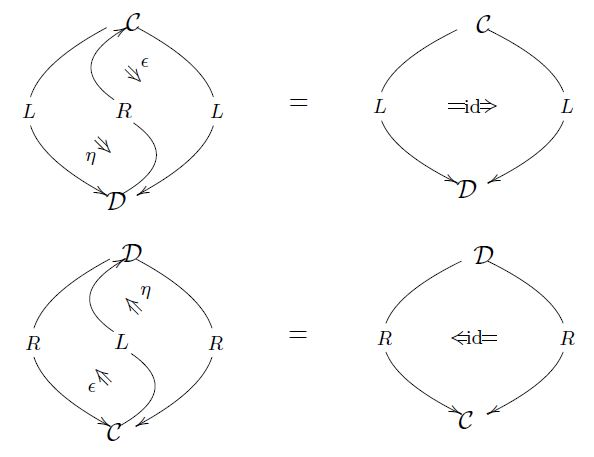
\includegraphics[width=7.5cm]{./media/Adjointness.jpg}
        \end{figure}
        \item[string diagram]
        "pulling the zigzag straight"の動きに対応する.
        \begin{figure}[h]
            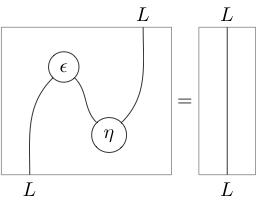
\includegraphics[width=3cm]{./media/adjunction-up-string.png}
            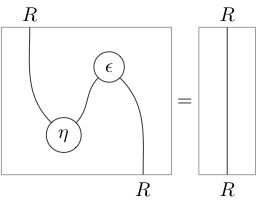
\includegraphics[width=3cm]{./media/adjunction-down-string.png}
        \end{figure}
    \end{description}
\end{remark}
\begin{remark}[unit, counit]
    歴史的にはunitはfront adjunctionと呼ばれていた.unitの由来は,任意の随伴に対して定まる$T:=R\circ L$はmonadであり,即ちmonoid objectの例であり,$\eta$がその単位射となっている.identity natural transformationのsynonymであるunitを取った.
\end{remark}
\begin{remarks}
    根底には群論や双線型形式を感じる.$A^*Q=PA$とは共軛$Q={}^t\!APA$のことである.
    diagramでの表記が後者で,hom-setに注目すると全射が見える.
    結局,一番下層で観測される事象は,An adjunct is given by precomposition with a unit or postcomposition with a counit.\footnote{\url{https://ncatlab.org/nlab/show/unit+of+an+adjunction}}
\end{remarks}

\begin{example}[adjunction]\mbox{}
    \begin{enumerate}
        \item Catの関手の組$(L,R)$がadjunctならば,それぞれをadjoint functorと呼ぶ.
        \item モノイド圏$A$に対して,単一対象な2-圏$\B A$の1-射は$A$の対象に対応する.この時,$\B A$のadjoint morphismの概念は,$A$におけるdualizing objectの概念に一致する.
    \end{enumerate}
\end{example}

\section{完備化}

\begin{tcolorbox}[colframe=ForestGreen, colback=ForestGreen!10!white,breakable,colbacktitle=ForestGreen!40!white,coltitle=black,fonttitle=\bfseries\sffamily,
title=]
    距離空間,測度空間,環に完備化が考えられるが,その名前は構成されるモノ射の性質による.
    後二者は代数的にも同じである.
\end{tcolorbox}

\begin{definition}[reflective, reflector / reflection, completion]\mbox{}
    \begin{enumerate}
        \item 充満忠実な部分圏$i:C\mono D$が\textbf{反射的}であるとは,この包含関手$i$が左随伴$T$を持つことをいう.この左随伴$T$を\textbf{反射(子)}という.
        \item 反射子$T$が忠実である時,\textbf{完備化}ともいう.
        \item 射$d\mono T(d)\in C$は冪等であり:$\forall_{c\in C}\;Tc\simeq c$(特徴付け\ref{lemma-characterization-of-reflector}より),
        この$T(d)\in C$を$d\in D$の\textbf{完備化}という.
    \end{enumerate}
\end{definition}
\begin{example}\mbox{}
    \begin{enumerate}
        \item $i:\Ab\to\Grp$は反射的である.この左随伴$T:\Grp\to\Ab$を\textbf{アーベル化}という:$\Hom_\Ab(T(-),-)\simeq\Hom_\Grp(-,i(-))$.
        ただしアーベル化は商群による構成であるように,いくつかの群準同型を同一化してしまうから,反射子$T$は充満であるが忠実でない.よってアーベル化は群に性質を付与する行為ではあるが,群の完備化とは言わない.
        \item 一方で距離空間を完備化しても,射(等長写像)は落ちない(忠実であるが充満ではない).
    \end{enumerate}
\end{example}

\begin{lemma}[反射子の特徴付け]\label{lemma-characterization-of-reflector}
    次の条件は同値.
    \begin{enumerate}
        \item $T:D\to C$は反射子である:充満忠実な右随伴関手$i:C\mono D$を持つ.
        \item 余単位$\ep:Ti\to \id_D$は関手の射である.
        \item モナド$(iT,T\ep i,\eta)$は冪等であり,$i:C\mono D$は保守的であり,$T$は本質的に全射である.
    \end{enumerate}
\end{lemma}

\chapter{モナド}

\begin{quotation}
    1965から圏論研究の中心はモナドに移った.
\end{quotation}

\section{定義}

\begin{definition}[monad]
    圏$C$と自己関手$T:C\to C$と自然変換$\eta:1_C\to T,\mu:T^2\to T$について,$(T,\eta,\mu)$が\textbf{モナド}であるとは,次の2つの図式を可換にすることをいう.
    \[\xymatrix{
        T^3\ar[r]^-{T\circ\mu}\ar[d]_-{\mu\circ T}&T^2\ar[d]^-{\mu}\\
        T^2\ar[r]^-\mu&T
    }\quad\xymatrix{
        T\ar[r]^-{\eta\circ T}\ar[dr]_-T&T^2\ar[d]^-\mu&T\ar[l]_-{T\circ\eta}\ar[dl]^-T\\
        &T
    }\]
    $\eta$を単位,$\mu$を積と言い,それぞれの図式を結合律とユニタリ律という.
\end{definition}

\section{構成}

\begin{tcolorbox}[colframe=ForestGreen, colback=ForestGreen!10!white,breakable,colbacktitle=ForestGreen!40!white,coltitle=black,fonttitle=\bfseries\sffamily,
title=]
    モナドはコホモロジー論で早くから現れ,Kanの随伴関手の発見以来,全てのモナドは随伴対から生じることが予想されていたが,これにEilenberg-MooreとKleisliとが独立に解答を与えた.
\end{tcolorbox}

\subsection{Eilenberg-Mooreの構成}

\subsection{Kleisliの構成}

\chapter{極限}

\begin{quotation}
    Internalizationとenrichmentを考えたい.圏が持ち得る構成の型を考える.
    あり得る理論が出て来る.
    例えば群論は有限積を備える圏で展開できる.圏論は引き戻しを備える圏で展開できる.
    Lawvereの代数的理論を学びたい.特に,有限な極限を持つ圏は,ほとんどの代数学を展開できる.ただ測度論のように$P(X)$に迫るには$\sigma$-性や$\delta$-性が欲しい.
    \begin{quote}
        One of the most important observations of category theory is that large parts of mathematics can be internalized in any category with sufficient structure.\footnote{\url{https://ncatlab.org/nlab/show/internal+logic}}
    \end{quote}
    これをさらに進めればinternal logicの考え方に至る.この先が真に数学が生息する母なる大地だと感じる.
    基本的には,certain algebraic structures can be defined in any category equipped with a categorified version of the same structure, as with monoid objects in a monoidal category.\footnote{\url{https://golem.ph.utexas.edu/category/2008/12/the_microcosm_principle.html}}
    \begin{quote}
        We name this principle the microcosm principle, after the theory, common in pre-modern correlative cosmologies, that every feature of the microcosm (e.g. the human soul) corresponds to some feature of the macrocosm.\cite{John and James}
    \end{quote}
\end{quotation}

\begin{tcolorbox}[colframe=ForestGreen, colback=ForestGreen!10!white, breakable ,colbacktitle=ForestGreen!40!white, coltitle=black,fonttitle=\bfseries\sffamily,
    title=]
    Grothendieckがlimit existsをlimit is representableと表現したことは気になる.
\end{tcolorbox}

\section{limit}

\begin{tcolorbox}[colframe=ForestGreen, colback=ForestGreen!10!white, breakable ,colbacktitle=ForestGreen!40!white, coltitle=black,fonttitle=\bfseries\sffamily,
    title=]
    錐を可換に補完するもののなす圏の中の終対象=最大のものが極限である.
    圏論的に極限とは,the “most optimized solution” to the problem of finding such an objectという営みである.\footnote{\url{https://ncatlab.org/nlab/show/limit}}
    ホモトピー論と並行に考えられるという.In practice, it is possibly best thought of in the context of representable functors as a classifying space for maps into a diagram.

    表現可能関手による定義とuniversal coneによる定義がある.
\end{tcolorbox}

\subsection{極限・余極限の定義}

\begin{definition}[inverse system, inverse limit / projective limit, direct limit / inductive limit]
    $C$を圏とし,順序集合$I$を圏と考える.
    \begin{enumerate}
        \item 関手$I\to C$を$I$上の$C$の\textbf{逆系}という.
        \item 逆系$A:I\to C$に対して,対象$B\in C$と射の族$(p_i:B\to A_i)_{i\in I}$であって,$i,j\in I,i\le j$に対して射$f_{ij}:A_i\to A_j$と$\forall_{i\le j}\;f_{ij}\circ p_i=p_j$の関係を満たすものを,$B$から$A$への\textbf{射の逆系}とよび,$B\to A$で表す.\footnote{錐とも呼ぶ.}$B$から$A$への$C$の射の逆系全体のなす集合を$\Mor_{C,I}(B,A)$で表す.
        \item 逆系$A:I\to C$について,対象$B\in C^\op$を射の逆系の集合に写す前層$\Mor_{C,I}(-,A):C^\op\to\Set$が表現可能であるとき,関手$\Mor_{C,I}(-,A)$を表現する$C$の対象を$A$の\textbf{逆極限}とよび,$\varprojlim_{i\in I}A_i$で表す.
        \item 極限$\varprojlim$を\textbf{射影極限}または\textbf{逆極限}という.余極限$\varinjlim$を\textbf{帰納極限}または\textbf{順極限}という.
    \end{enumerate}
\end{definition}
\begin{remark}
    極限とは違う用語を使うことは,図式の始域$I$を有向集合や順序集合に制限する代数学の流れを汲んでいる.
    むしろこちらの方が圏論的な定義が与えられる前の定義であった.
\end{remark}

\begin{definition}[constant inverse system]\mbox{}
    \begin{enumerate}
        \item $A_i:=A\;(i\in I),f_{ij}:=1_A\;(i\le j)$として定まる$C$の逆系を\textbf{定数逆系}といい,$A_I$で表す.
        \item 射の逆系$B\to A$とは,逆系の圏$\Fun(I,C)$での定数逆系からの射$B\to A$のこととみなせる.
        \item 逆系$A:I\to C$の逆極限$\varprojlim_{i\in I}A_i\in C$は,射の逆系$\varprojlim_{i\in I}A_i\to A$であって,$C$の任意の対象に対して写像$\Mor_C(B,\varprojlim_{i\in I}A_i)\to\Mor_{C,I}(B,A)$が可逆になるようなものが存在する$C$の対象である.これを逆極限の\textbf{普遍性}という.
        \item $j\in I$に対し,標準射の逆系$\varprojlim_{i\in I}A_i\to A$の成分$p_j:\varprojlim_{i\in I}A_i\to A_j$を\textbf{射影}という.
    \end{enumerate}
\end{definition}
\begin{example}
    $I$を順序集合とする.
    \begin{enumerate}
        \item $I=\emptyset$について,空な族の逆極限$\varprojlim_{i\in\emptyset}A_i$は$C$の終対象である.
        \item $A$を集合の逆系とすると,$\varprojlim_{i\in I}A_i=\Brace{(x_i)\in\prod_{i\in I}A_i\;\middle|\;i\le j\Rightarrow x_j=f_{ij}(x_i)}$.
        \item $M$を可換群の逆系とする.集合としての逆極限$\varprojlim_{i\in I}M_i$は,成分ごとの演算が定める積群$\prod_{i\in I}M_i$の部分群であり,可換群としての逆極限である.
    \end{enumerate}
\end{example}

\begin{proposition}
    $A$を圏$C$の逆系,$B\in C$を対象とする.\[\Mor_{C,I}(B,A)=\varprojlim_{i\in I}\Mor_C(B,A_i).\]
\end{proposition}

\begin{proposition}
    $C$の任意の逆系に対し逆極限が存在するならば,$C$の逆系を逆極限に写す関手$\varprojlim_{i\in I}:\Fun(I,C)\to C$は,$C$の対象を定数逆系に写す関手$(-)_{i\in I}:C\mono\Fun(I,C)$の右随伴関手となる.
\end{proposition}

\subsection{有向集合論}

\begin{definition}[もう一つの射影]
    順序写像$f:J\to I$に対して,precompositionが定める逆系のなす圏の関手$f^*:\Fun(I,C)\to\Fun(J,C)$が考えられる.
    逆系$A:I\to C$に対して,これは前層の射$\Mor_{C,I}(-,A)\to\Mor_{C,J}(-,f^*A)$を定める.
    $A$と$f^*A$に逆極限が存在すれば,これは逆極限の普遍性から,射$\varprojlim_{i\in I}A_i\to\varprojlim_{j\in J}A_{f(j)}$を定める.
    $i:J\mono I$については,$f^*A$を$A|_J$で表し,射$\varprojlim_{i\in I}A_i\to\varprojlim_{j\in J}A_{f(j)}$も\textbf{射影}と呼ぶ.
\end{definition}

\begin{definition}[(downward) filtered / directed, cofinal]
    $I$を順序集合とする.
    \begin{enumerate}
        \item $I\ne\emptyset$であり,$\forall_{i,j\in I}\;\exists_{k\in I}\;k\le i\land k\le j$が成り立つとき,$I$を\textbf{有向}であるという.
        \item 部分集合$J\subset I$が$\forall_{i\in I}\;\exists_{j\in J}\;j\le i$を満たすとき,$J$は\textbf{共終}であるという.
    \end{enumerate}
\end{definition}
\begin{example}
    位相空間$X$について,
    \begin{enumerate}
        \item $x$の近傍系$N(X,x)$は有向集合である.
        \item 部分集合$M\subset N(X,x)$が基本系であるとは,共終であることをいう.
        \item $x$の開近傍全体がなす集合$M(X,x)$は$N(X,x)$の共終な部分集合である.
    \end{enumerate}
\end{example}

\begin{proposition}
    $I$を有向集合とし,$J\subset I$をその共終な部分集合とする.
    \begin{enumerate}
        \item $J$も有向である.
        \item 任意の$i\in I$に対して$J_i:=\Brace{j\in J\mid j\le i}$は$I$の共終な部分集合である.
    \end{enumerate}
\end{proposition}
\begin{proof}\mbox{}
    \begin{enumerate}
        \item $I\ne\emptyset$であることより,$J\ne\emptyset$である.任意の$j,j'\in J$に対して,$I$は有向だから$i\in I$が存在して$i\le j,i\le j'$を満たす.$J$は共終だから,$\exists_{k\in J}\;k\le i$を満たす.
        \item 任意の$i\in I$に対して,任意の$k\in I$を取る.$I$は有向だから,$\exists_{l\in I}\;l\le i,k$で,$J$は共終だから$\exists_{j\in I}\;j\le l$.すると$j\le l\le i$だから$j\in J_i$であり,かつ,$j\le l\le k$より,共終である.
    \end{enumerate}
\end{proof}

\subsection{逆極限の存在条件}

\begin{proposition}
    $C$を圏とし,$A$を有向集合$I$上の$C$の逆系とする.
    \begin{enumerate}
        \item (coneは同じだけある) $J$が$I$の共終な部分集合ならば,$C$上の前層の射$\Mor_{C,I}(-,A)\to\Mor_{C,J}(-,A|_J)$は同型である.
        \item 逆極限$\varlim_{j\in J}A_j$が存在すれば,$\varlim_{i\in I}A_i$も存在し,射影$\varlim_{i\in I}A_i\to\varlim_{j\in J}A_j$は同型である.
    \end{enumerate}
\end{proposition}

\begin{proposition}
    $I$を有向集合とし,$C$を圏とする.
    \begin{enumerate}
        \item $C$の対象$A$を定数逆系に写す関手$i:C\mono\Fun(I,C)$は充満忠実である.
        \item $C$の逆系$A\in\Fun(I,C)$に対して,次の2条件は同値:
        \begin{enumerate}[(a)]
            \item 任意の$i\le j$に対して$f_{ij}:A_i\to A_j$は同型.
            \item $C$の対象$B$が存在して,その定数逆系からの同型$B_I\to A$が存在する.
        \end{enumerate}
        \item $C$の逆系$A\in\Fun(I,C)$が(2)の(a)の条件を満たすならば,逆極限$\varlim_{i\in I}A_i$は存在し,任意の$j\in I$に対して$\varlim_{i\in I}A_i\to A_j$は同型である.
    \end{enumerate}
\end{proposition}

\section{pullback}

\begin{tcolorbox}[colframe=ForestGreen, colback=ForestGreen!10!white, breakable ,colbacktitle=ForestGreen!40!white, coltitle=black,fonttitle=\bfseries\sffamily,
    title=pullback is limit over a cospan]
    引き戻しと座標変換.
\end{tcolorbox}

\begin{definition}\mbox{}
    \begin{enumerate}
        \item 図式
        \[\xymatrix{
            a\ar[dr]_-f&&b\ar[dl]^-g\\
            &c
        }\]
        をpullback diagramまたはcospanという.
        \item pullbackとは,cospanの
        の極限である.
        \item 出来上がる四角形の図式をpullback squareと呼ぶ.
        \item 反対圏$C^\op$でのpullbackをpushoutと呼ぶ.
    \end{enumerate}
\end{definition}

\begin{proposition}[等化子としての特徴付け]
    $C$は積を備えるとする.引き戻し
    \[\xymatrix{
        a\times_cb\ar[r]\ar[d]&a\ar[d]^-f\\
        b\ar[r]_-g&c
    }\]
    は,$f,g$が積$a\times b$に沿って定める射についての等化子
    \[\xymatrix@1{
        a\times_cb\ar[r]&a\times b\ar@/^/[r]^-{f\pr_1}\ar@/_/[r]_-{g\pr_2}&c
    }\]
\end{proposition}

\begin{proposition}[引き戻しはmono, isoを保存する]
    \[\xymatrix{
        a\ar[r]\ar[d]_-{f^*g}&b\ar[d]^-g\\
        c\ar[r]_-f&d
    }\]
    をpullback squareとする.
    \begin{enumerate}
        \item $g$がmonicならば,$f^*g$もmonicである.
        \item $g$が同型ならば,$f^*g$も同型である.
    \end{enumerate}
    逆はいずれも成り立たない.
\end{proposition}

\begin{proposition}[pasting law for pullbacks]
    次の可換図式を考える.
    \[\xymatrix{
        a\ar[r]\ar[d]&b\ar[r]\ar[d]&c\ar[d]\\
        d\ar[r]&e\ar[r]&f
    }\]
    right-hand inner squareがpullbackであるとする.left-hand inner squareがpullbackであることと,outer squareがpullbackであることは同値.
\end{proposition}
\begin{remark}
    left-hand inner squareとouter squareがpullbackであるのに,right-hand inner squareはpullbackではない例が存在する.
\end{remark}

\begin{definition}[base change morphism / pullback functor]
    引き戻しを備える圏$C$について,$f:X\to Y$を射とする.
    これは,over category上に,引き戻し関手$f^*:C/Y\to C/X$を引き起こす.
    これを\textbf{基底変換射}という.
\end{definition}

\section{Kan拡張}



\begin{thebibliography}{9}
    \bibitem{数学原論}
    斎藤毅『数学原論』(2020)
    \bibitem{John and James}
    John C. Baez, James Dolan, Higher-Dimensional Algebra III: n-Categories and the Algebra of Opetopes (1997)
    \bibitem{Mac Lane}
    Sanders Mac Lane "Category for the Working Mathematicians" (98)
    \bibitem{大熊}
    大熊正 (1979) 『圏論』(数学選書,槙書店).
\end{thebibliography}

\end{document}